\documentclass[12pt,a4paper]{ctexart}
\usepackage[a4paper,margin=2.2cm]{geometry}
\usepackage{graphicx}
\usepackage{booktabs}
\usepackage{float}
\usepackage{enumitem}
\usepackage{array}
\usepackage{longtable}
\usepackage{amsmath}
\usepackage{caption}
\captionsetup{font=small}
\graphicspath{{../result/}{result/}}

\begin{document}

\begin{center}
{\LARGE \textbf{上机实验报告——回归模型与模型评估}}\\[1em]
学号：1043220122 \hspace{2cm} 姓名：林鑫
\end{center}

\vspace{1em}

\section*{一、实验目的}
\begin{enumerate}[label=（\arabic*）]
\item 掌握线性正则化模型：理解并实现岭回归（Ridge）、Lasso 回归和 ElasticNet 回归，掌握 L1 与 L2 正则化在防止过拟合和处理多重共线性中的作用。
\item 掌握强力 Boosting 算法：学会使用 XGBoost 进行回归任务，理解其迭代纠错的核心原理。
\item 理解集成学习的思想：掌握 Voting（投票）与 Stacking（堆叠）两种集成策略，通过组合多个基模型提升预测精度和稳定性。
\item 完成模型对比与评估：能够比较不同回归模型在相同数据集上的表现，并结合结果分析模型的适用场景。
\end{enumerate}

\section*{二、实验环境}
\begin{enumerate}[label=（\arabic*）]
\item 编程语言：Python
\item 核心库：
\end{enumerate}

\noindent pandas、numpy：数据读取、数据清洗与数值计算\\
\noindent sklearn：数据预处理、模型构建、正则化回归、集成学习与模型评估\\
\noindent xgboost：XGBoost 回归模型\\
\noindent matplotlib、seaborn：数据可视化与结果展示

\section*{三、实验数据介绍（对使用数据集作介绍）}
本实验使用的数据文件为 \texttt{code/沪深300\_最近三年.csv}，数据内容为沪深300指数近三年的日线交易记录。原始数据共 727 条样本，时间范围为 2023-03-27 至 2026-03-27，包含日期、收盘价、开盘价、最高价、最低价、交易量和涨跌幅 7 个原始字段。

结合实验任务，本次作业以“收盘价”作为回归目标变量，其余价格类字段、成交量字段以及基于时间顺序构造的历史特征作为输入变量。与实验三保持一致，本文在原始字段基础上进一步构造了年、月、日、星期、价格振幅、开高差、开低差、高低比、日内振幅率、成交量变化率、3/5/10 日滚动均值、5 日收益波动，以及 1/2/3/5 日滞后特征，从而增强模型对价格变化规律的表达能力。

需要特别说明的是，原始字段中的“涨跌幅”由收盘价相对前一交易日收盘价计算得到，因此如果直接把当日涨跌幅作为输入，会带来目标泄漏风险。为避免该问题，实验中仅保留其滞后项参与建模。经过缺失值处理、异常值截尾和滚动特征构造后，最终可用于实验建模的样本数为 716 条。

\section*{四、实验内容与步骤}

\subsection*{1. 数据加载与预处理（读取数据集、处理缺失值、异常值、重复行，并说明标准化处理）}
首先读取 CSV 文件，并将日期字段转换为日期类型，再按照时间先后顺序排序。随后将交易量中的 \texttt{K} 去除并转换为数值型，将涨跌幅中的百分号去除并转换为浮点型，便于后续计算和建模。检查结果表明，原始数据中仅存在 1 条缺失记录，且集中在涨跌幅字段；重复行数量为 0，因此本文直接删除缺失样本并保留其余有效数据。

在异常值处理方面，本文延续实验三的思路，使用 IQR（四分位距）方法对收盘价、开盘价、最高价、最低价、交易量和涨跌幅六个数值字段进行检测，并采用截尾（clip）方式降低极端值对回归模型训练的影响。检测结果显示，异常值相对较多的字段为：pct\_change（29 个）、volume（20 个），其余字段异常值数量较少。从金融数据特点来看，这类异常值通常反映的是阶段性急涨急跌或交易放量现象，并不一定是错误数据，因此实验中未直接删除，而是通过截尾方式保留总体趋势、削弱极端扰动。

在完成清洗后，进一步进行特征工程。除原始价格字段外，增加了日历特征（年、月、日、星期）、价格差分特征（振幅、开高差、开低差）、比例特征（高低比、日内振幅率）、成交量变化特征、滚动均值特征（3 日、5 日、10 日均线）以及滞后特征（前 1/2/3/5 日价格与成交量信息）。这些特征一方面能增强模型的解释能力，另一方面也为 Lasso、ElasticNet 和集成模型提供更丰富的输入空间。

\begin{figure}[H]
\centering
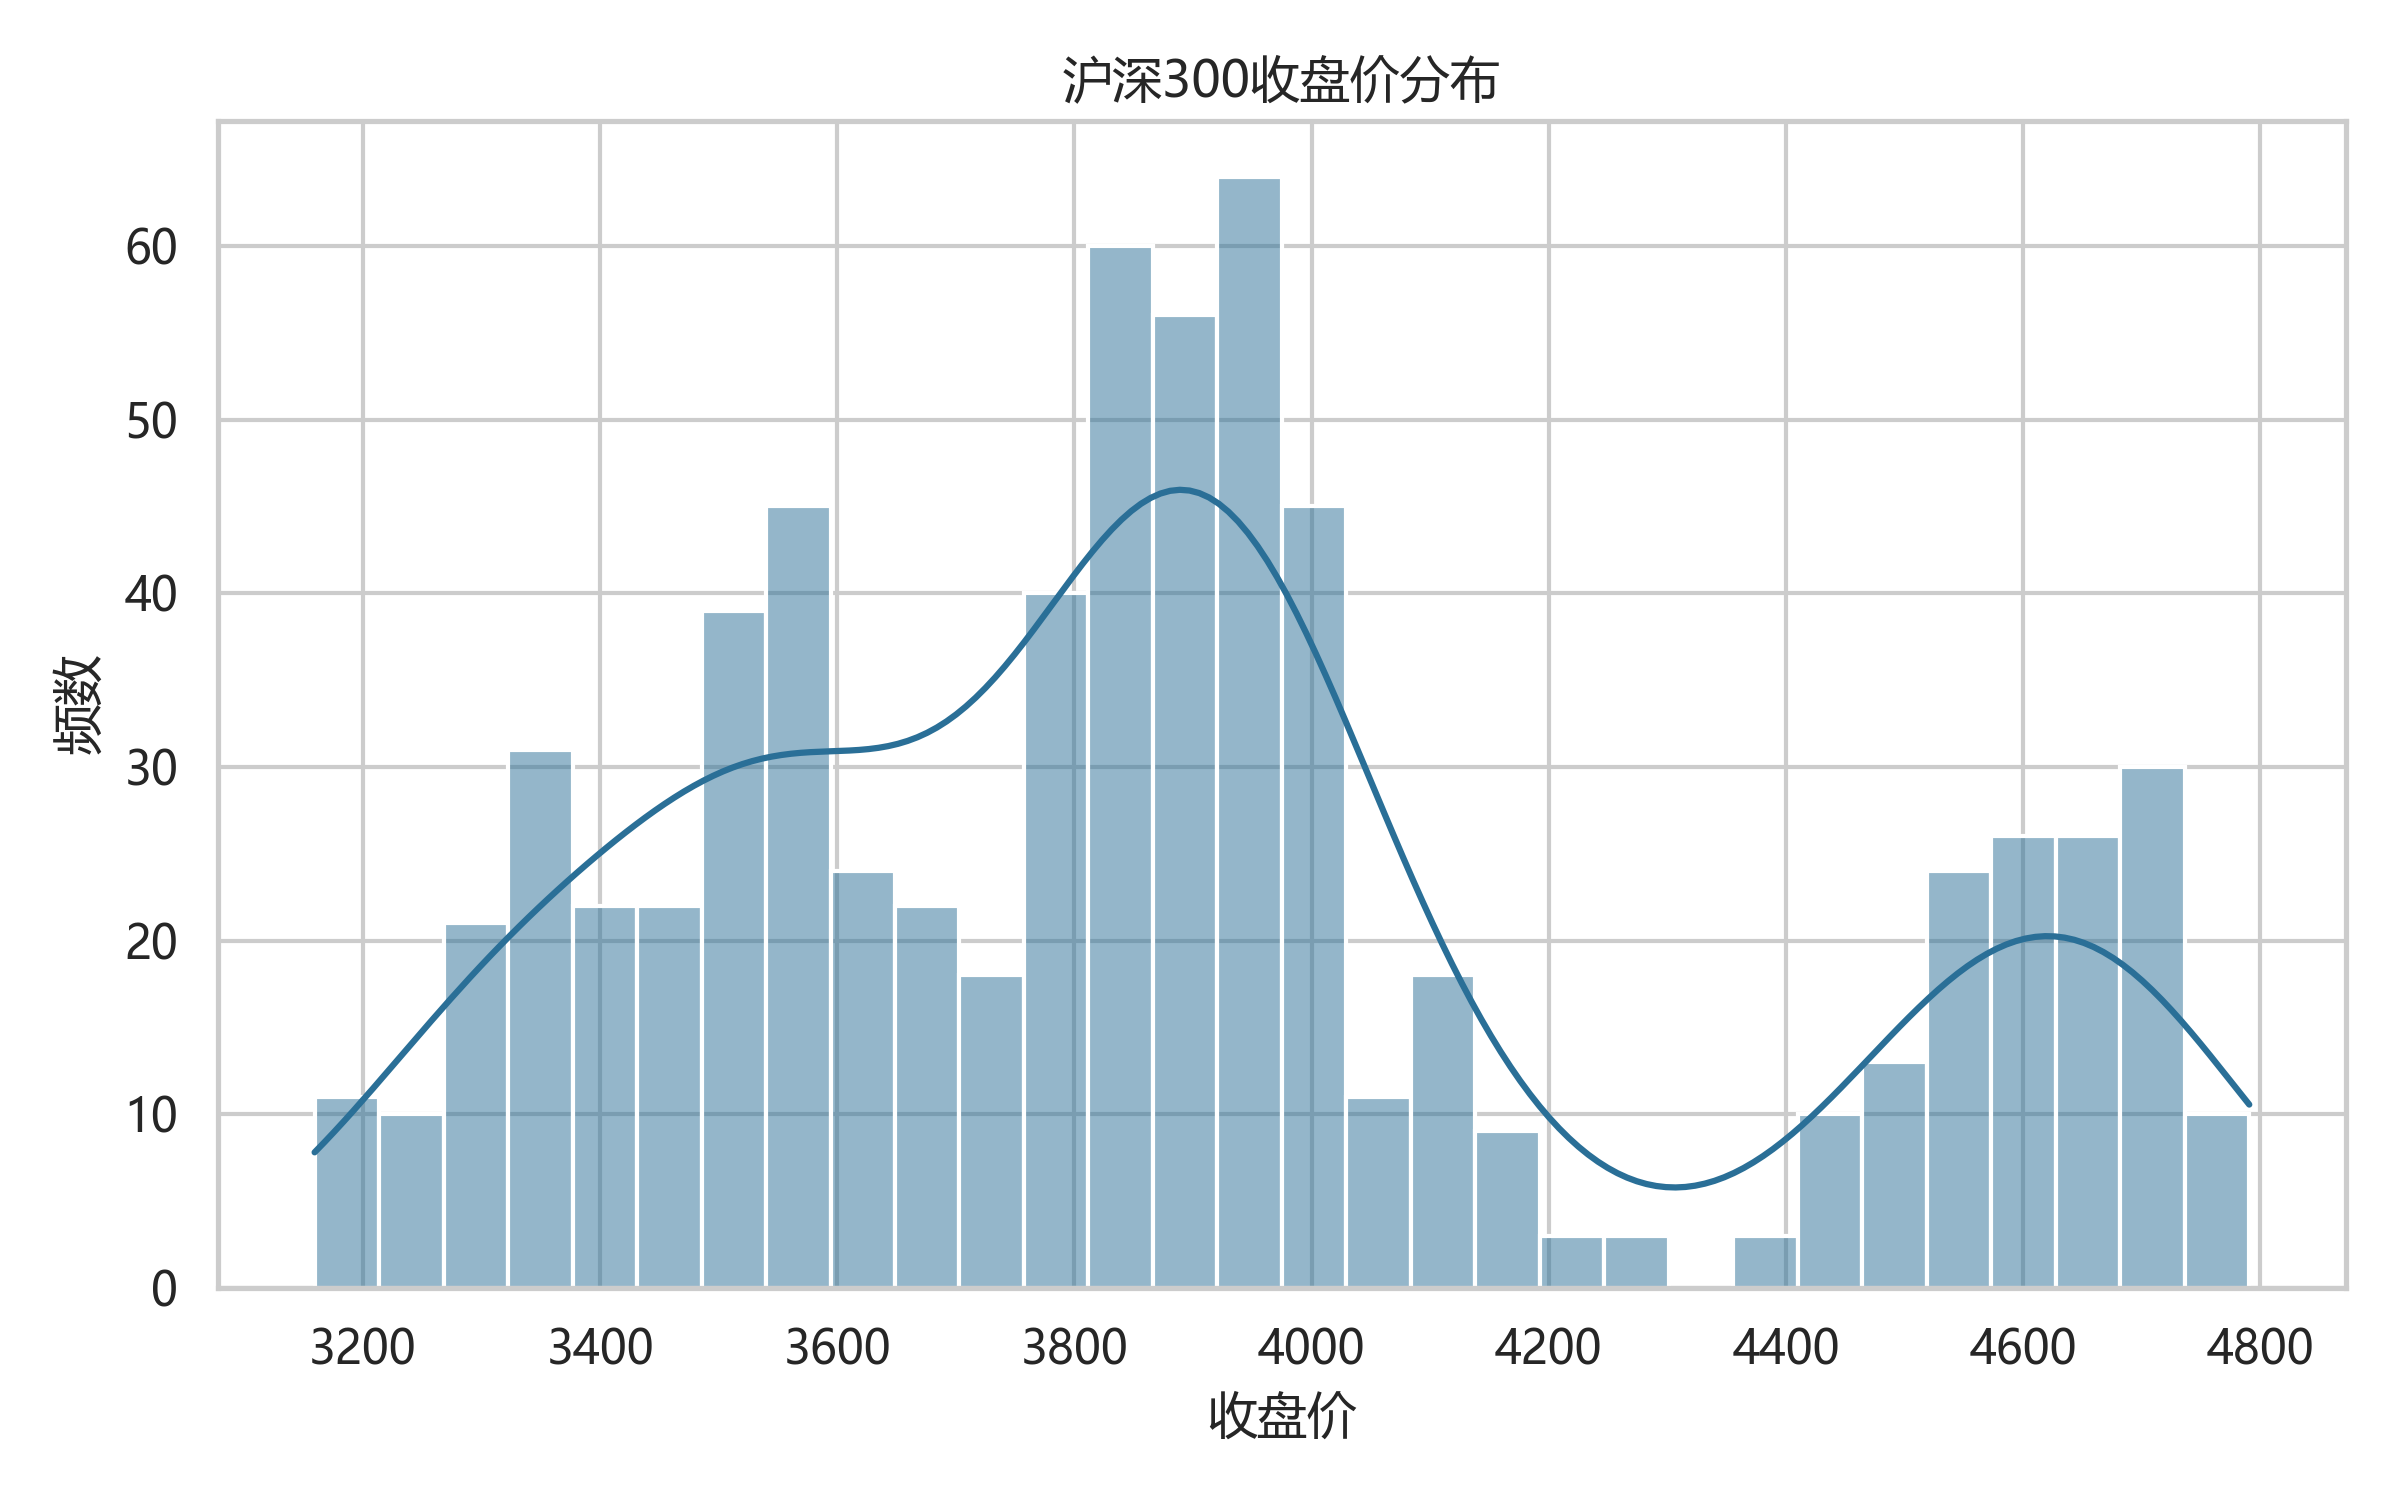
\includegraphics[width=0.92\textwidth]{01_close_distribution.png}
\caption{收盘价分布图}
\end{figure}

\begin{figure}[H]
\centering
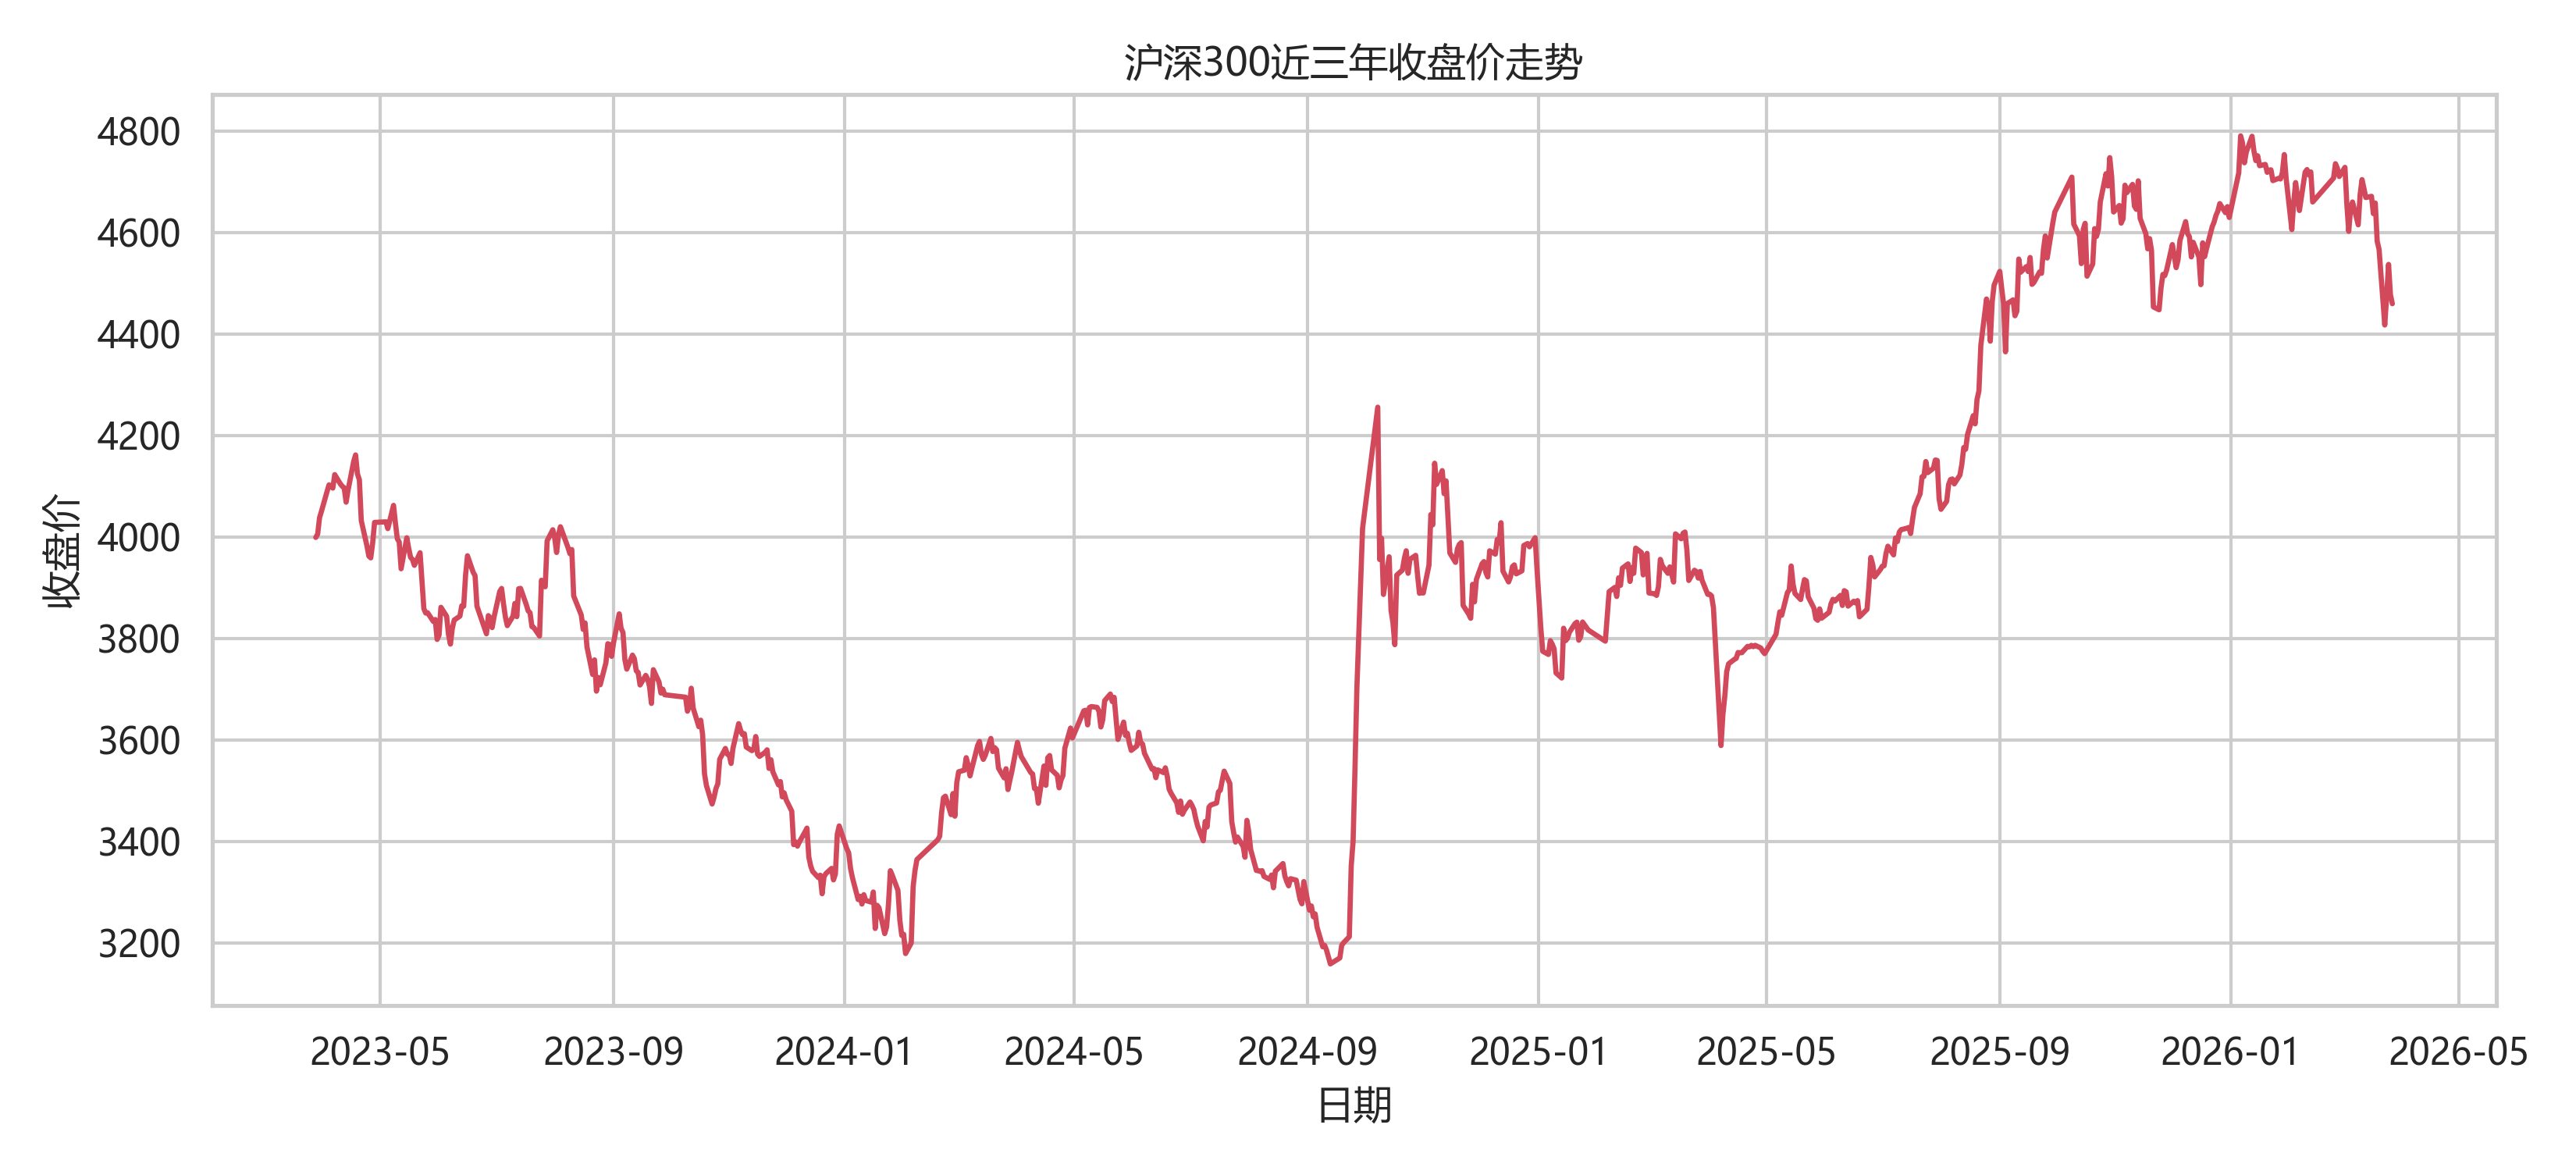
\includegraphics[width=0.92\textwidth]{02_close_trend.png}
\caption{沪深300近三年收盘价走势}
\end{figure}

\begin{figure}[H]
\centering
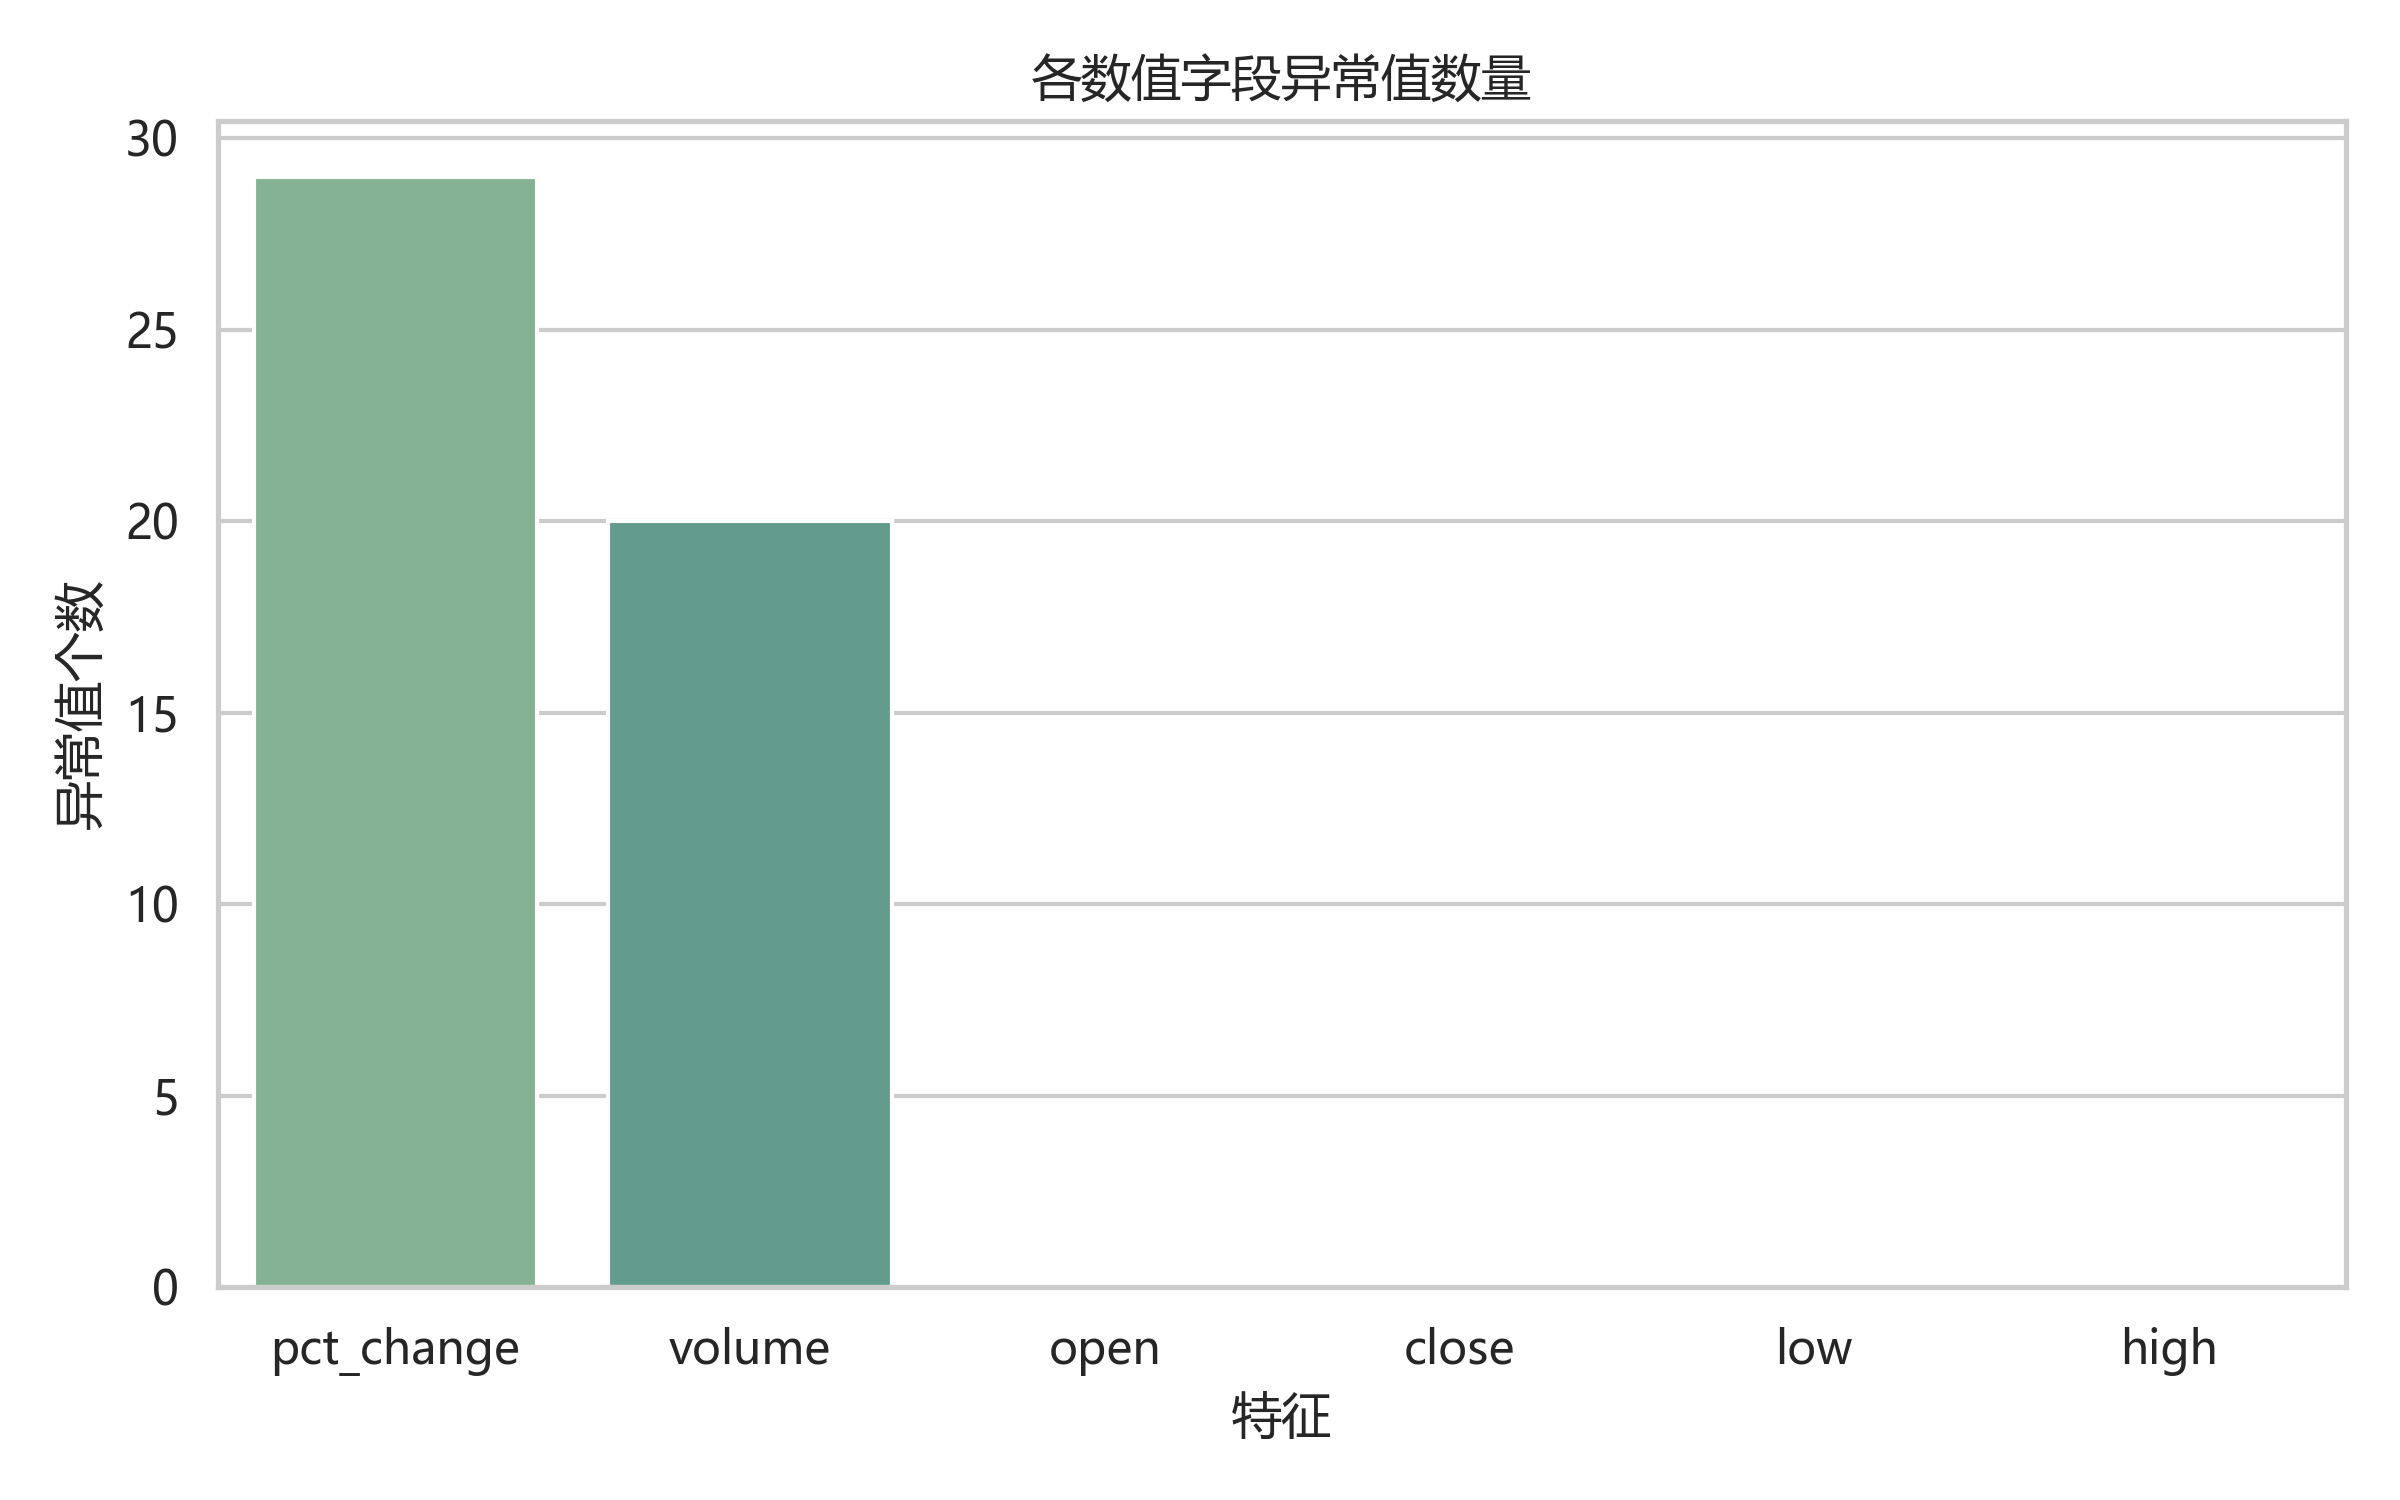
\includegraphics[width=0.80\textwidth]{04_outlier_counts.png}
\caption{各数值字段异常值统计}
\end{figure}

由于岭回归、Lasso 和 ElasticNet 等正则化模型对特征尺度非常敏感，如果不同特征数量级差异过大，正则化惩罚项就无法对各个系数进行公平约束，因此必须进行标准化处理。本文在训练集上使用 \texttt{StandardScaler} 拟合均值和标准差，再把同样的变换应用到训练集和测试集。图~\ref{fig:std-compare} 展示了标准化前后部分特征分布的变化情况，可以看到标准化后各特征的尺度更加统一，数值整体集中在 0 附近，有利于正则化模型稳定收敛。

\begin{figure}[H]
\centering
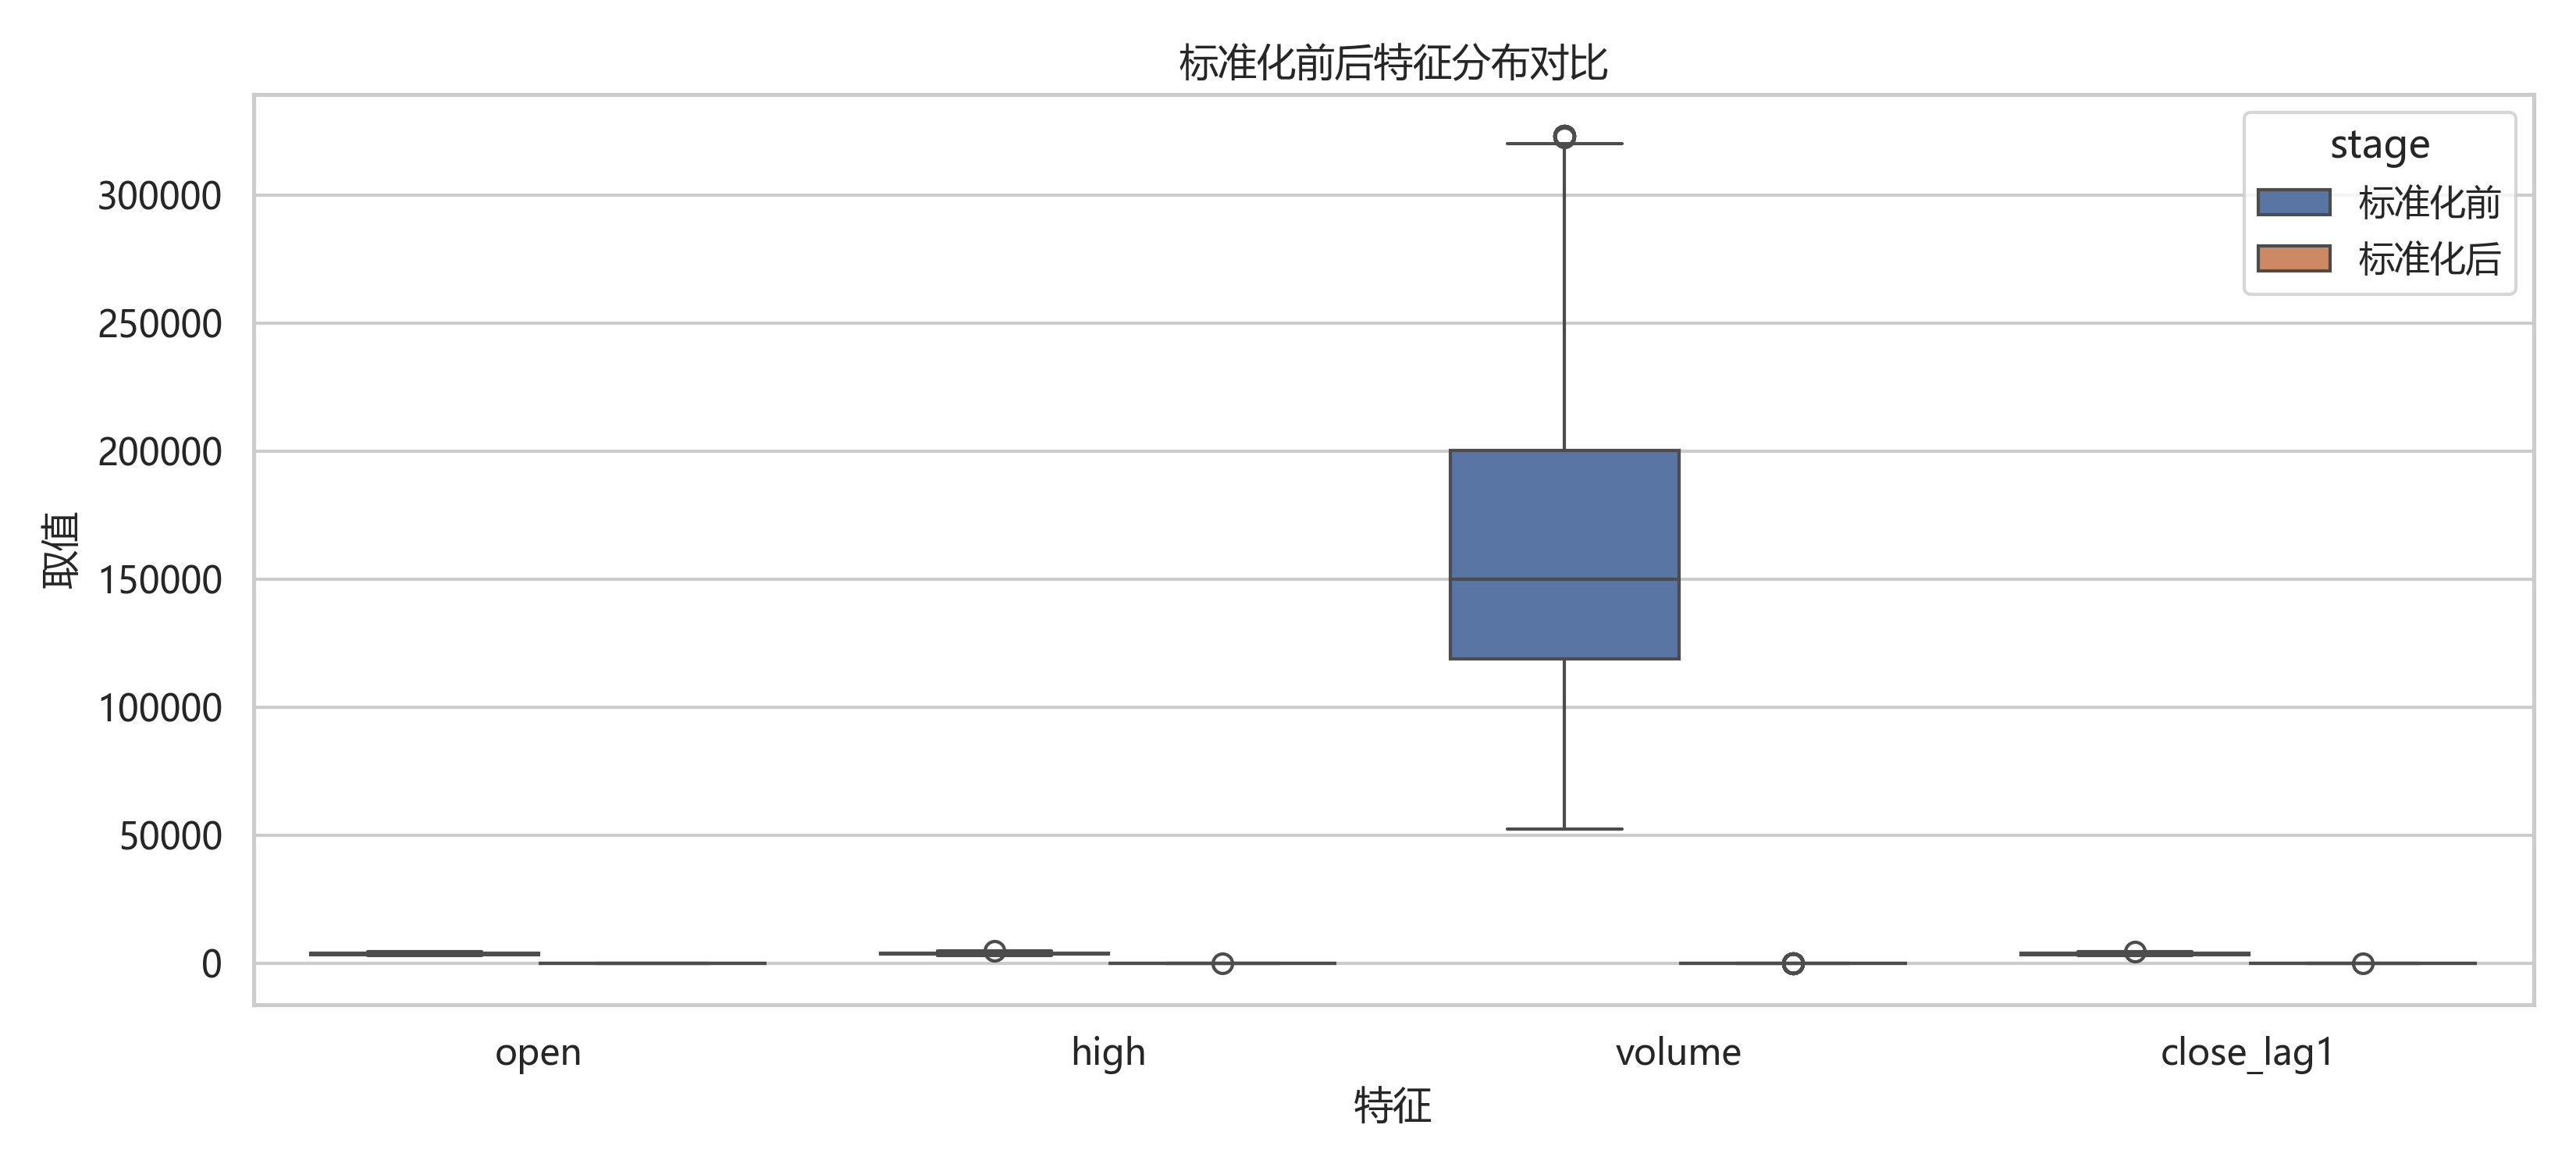
\includegraphics[width=0.90\textwidth]{05_standardization_compare.png}
\caption{标准化前后特征分布对比}
\label{fig:std-compare}
\end{figure}

\subsection*{2. 数据集划分（训练集与测试集划分）}
本实验采用常见的训练集 80\%、测试集 20\% 的划分方式，对全部建模样本进行切分。其中训练集样本数为 572，测试集样本数为 144，对应比例分别约为 80% 和 20%。考虑到本次实验的重点是比较多种回归模型在同一数据集上的表现，因此这里采用固定随机种子 \texttt{random\_state=42} 的随机划分方式，以保证不同模型使用完全一致的训练样本与测试样本，确保结果具有可比性。

划分完成后，将训练集特征矩阵输入 \texttt{StandardScaler} 进行拟合，得到标准化后的训练集和测试集，再用于后续所有模型训练和预测。这样做可以使普通线性回归和各类正则化回归在统一尺度下比较，也便于 Voting 与 Stacking 中不同基模型之间的组合。

\subsection*{3. 构建与训练回归模型}
本实验共构建了 8 种回归模型，分别为普通线性回归（Linear）、Ridge 回归、Lasso 回归、ElasticNet 回归、支持向量回归（SVR）、XGBoost 回归、Voting 回归和 Stacking 回归。其中，普通线性回归作为基准模型，用于衡量不加正则化时的拟合效果；Ridge 通过 L2 正则化缓解共线性；Lasso 通过 L1 正则化实现特征筛选；ElasticNet 结合 L1 与 L2 正则化；XGBoost 用于测试非线性树模型在该数据集上的效果；Voting 和 Stacking 则用于验证集成学习策略对精度与稳定性的提升作用。

各模型参数设置如下：Ridge 使用网格搜索在 $\alpha \in \{0.01, 0.1, 1, 10, 50, 100\}$ 中选取最优值，最终得到 $\alpha=0.1$；Lasso 的最优参数为 $\alpha=1.0$，非零系数数量为 6，说明在当前特征集合下 Lasso 保留了主要有效特征并对部分冗余变量进行了压缩；ElasticNet 的最优参数为 $\alpha=0.001$、\texttt{l1\_ratio}=0.9；SVR 的最优参数为 \texttt{C=50}、\texttt{epsilon=0.05}；XGBoost 采用 \texttt{n\_estimators=200}、\texttt{learning\_rate=0.05}、\texttt{max\_depth=4} 的参数组合。Voting 回归集成了 Ridge、Lasso、ElasticNet 和 SVR 四个模型；Stacking 回归第一层使用 Ridge、Lasso、XGBoost，第二层使用 Ridge 作为元模型。

为了让不同模型的预测效果比较更直观，除指标表外，实验还对所有模型在测试集上的预测结果进行了可视化。图~\ref{fig:model-predict-line} 给出了各模型在测试集上的“真实值-预测值”折线对比图，图~\ref{fig:model-predict-scatter} 给出了真实值与预测值的散点对比图。通过这两组图可以观察各模型对收盘价波动的跟踪程度和拟合偏差，其中线性正则化模型整体表现较为稳定，预测曲线与真实曲线贴合度较高，而 XGBoost 的离散误差相对更明显。

\begin{figure}[H]
\centering
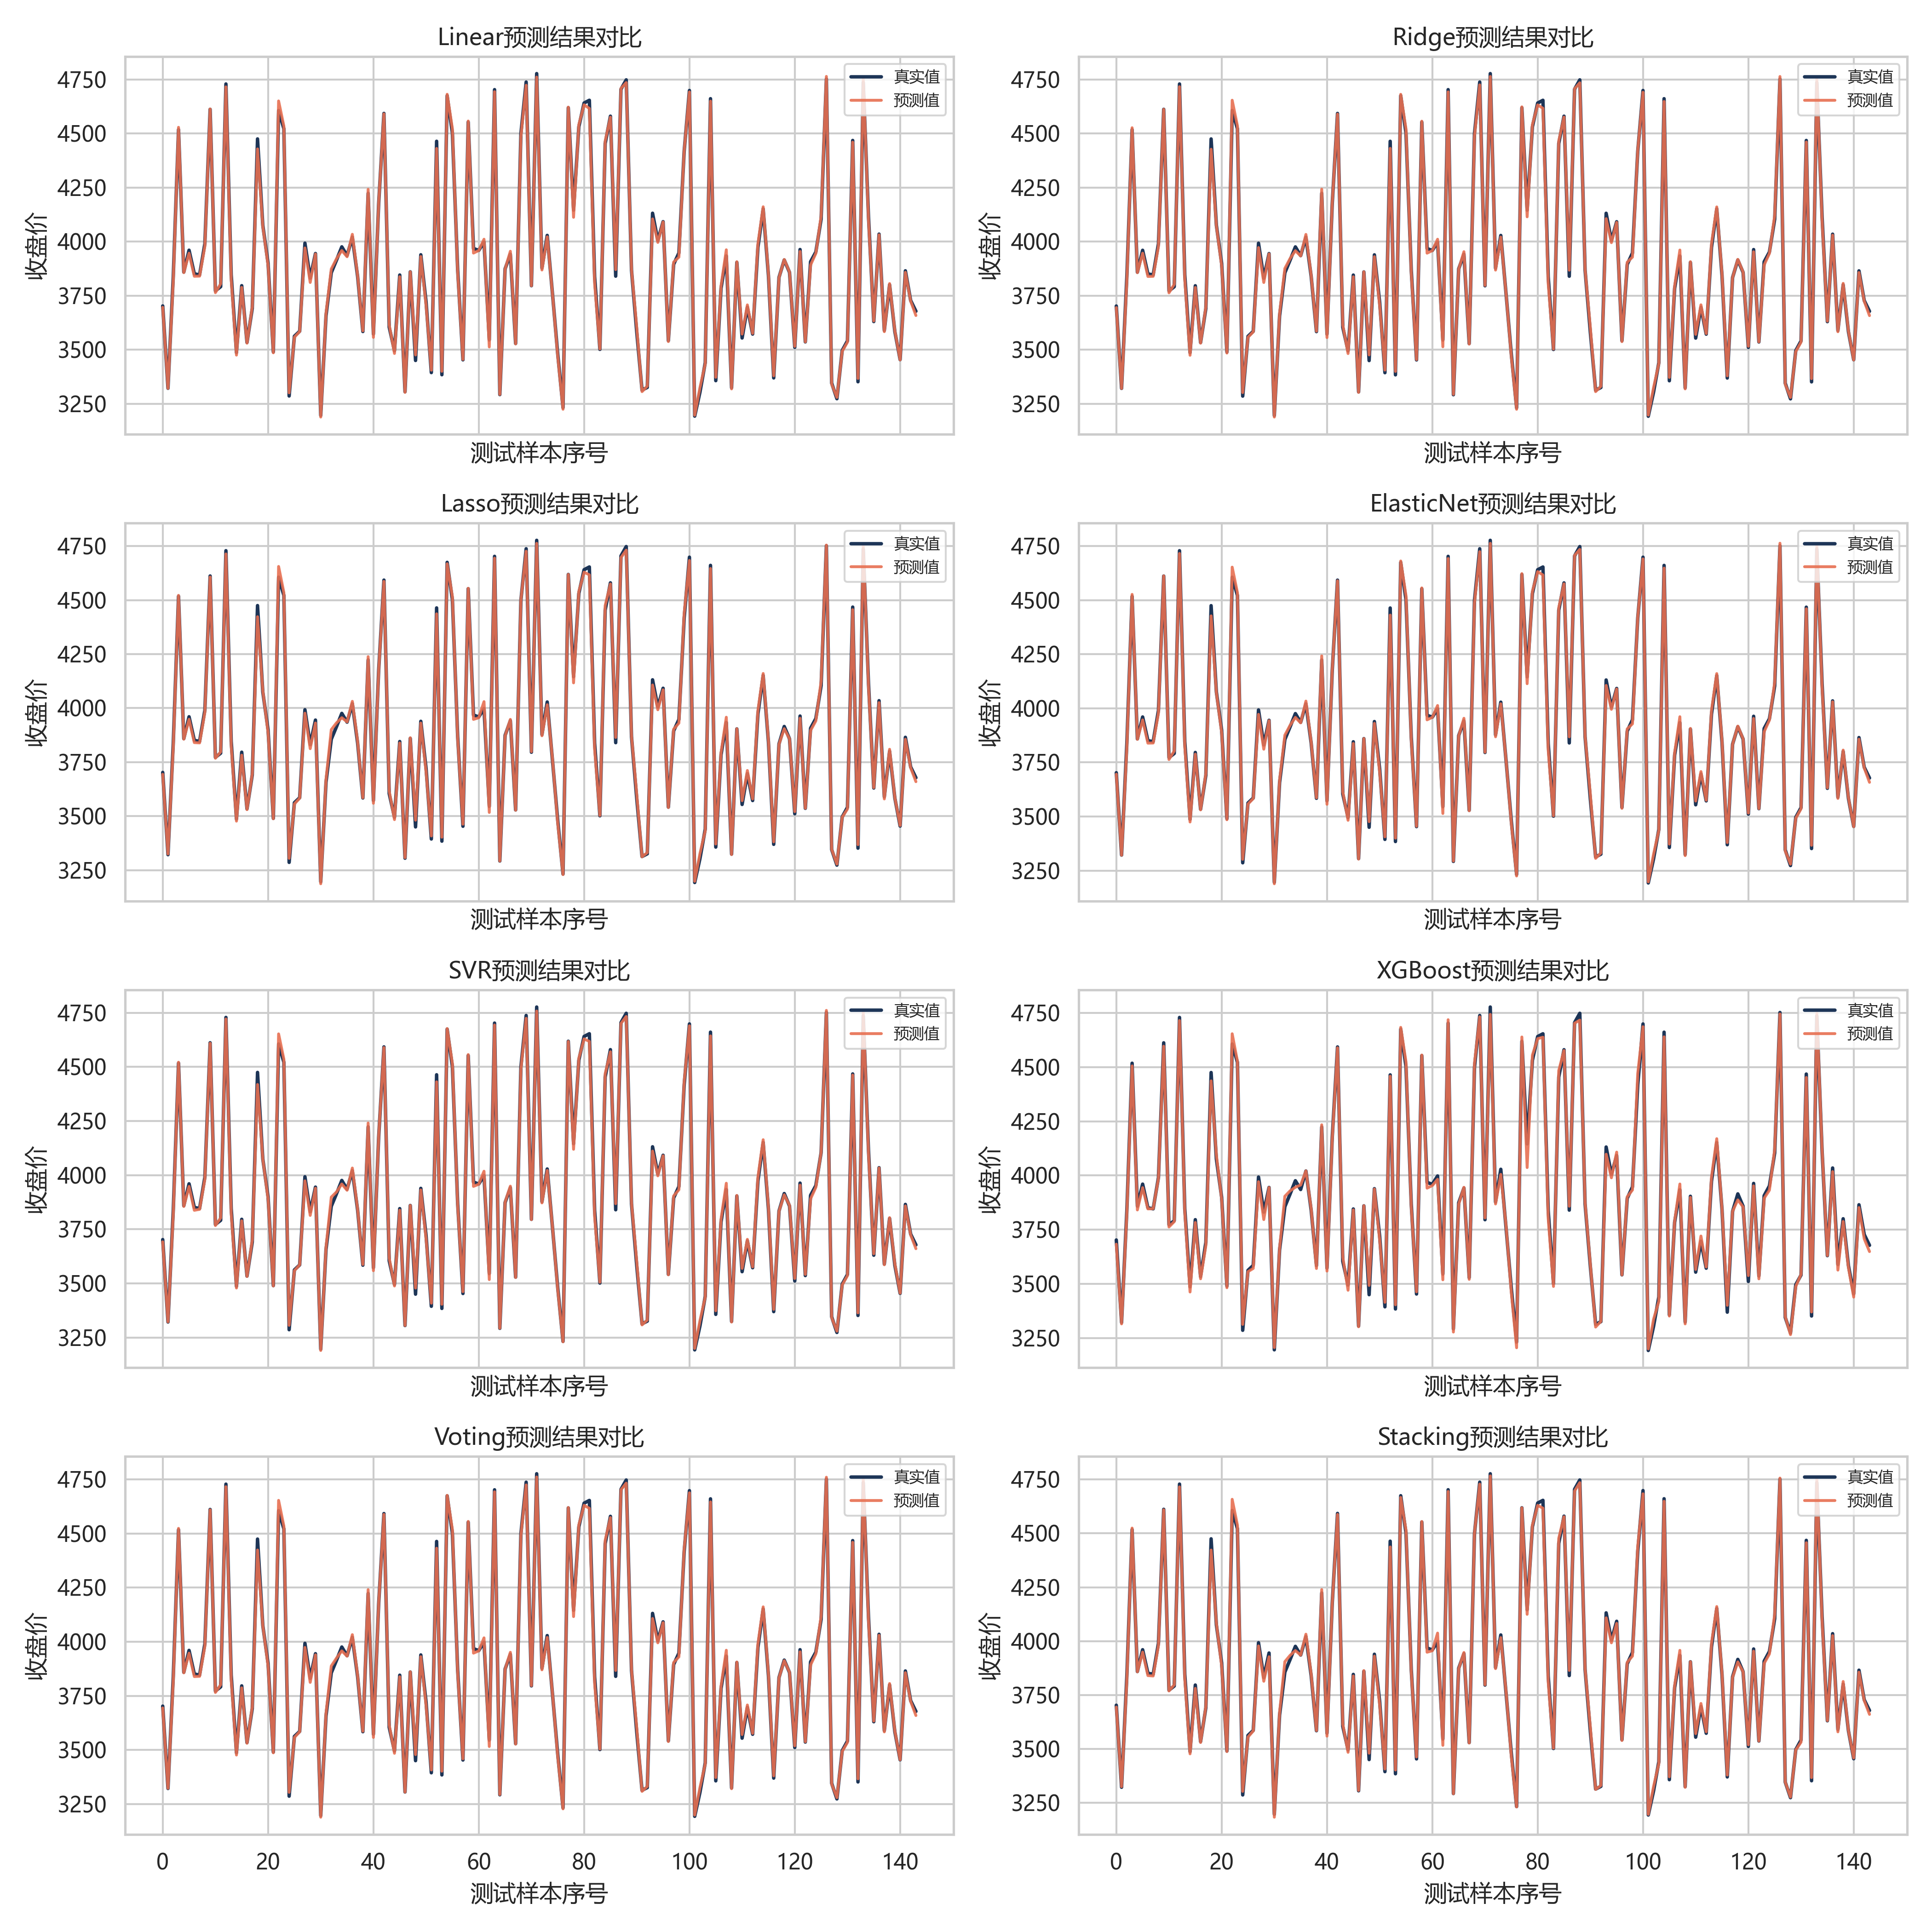
\includegraphics[width=0.94\textwidth]{08_model_prediction_compare.png}
\caption{各预测模型测试集折线对比}
\label{fig:model-predict-line}
\end{figure}

\begin{figure}[H]
\centering
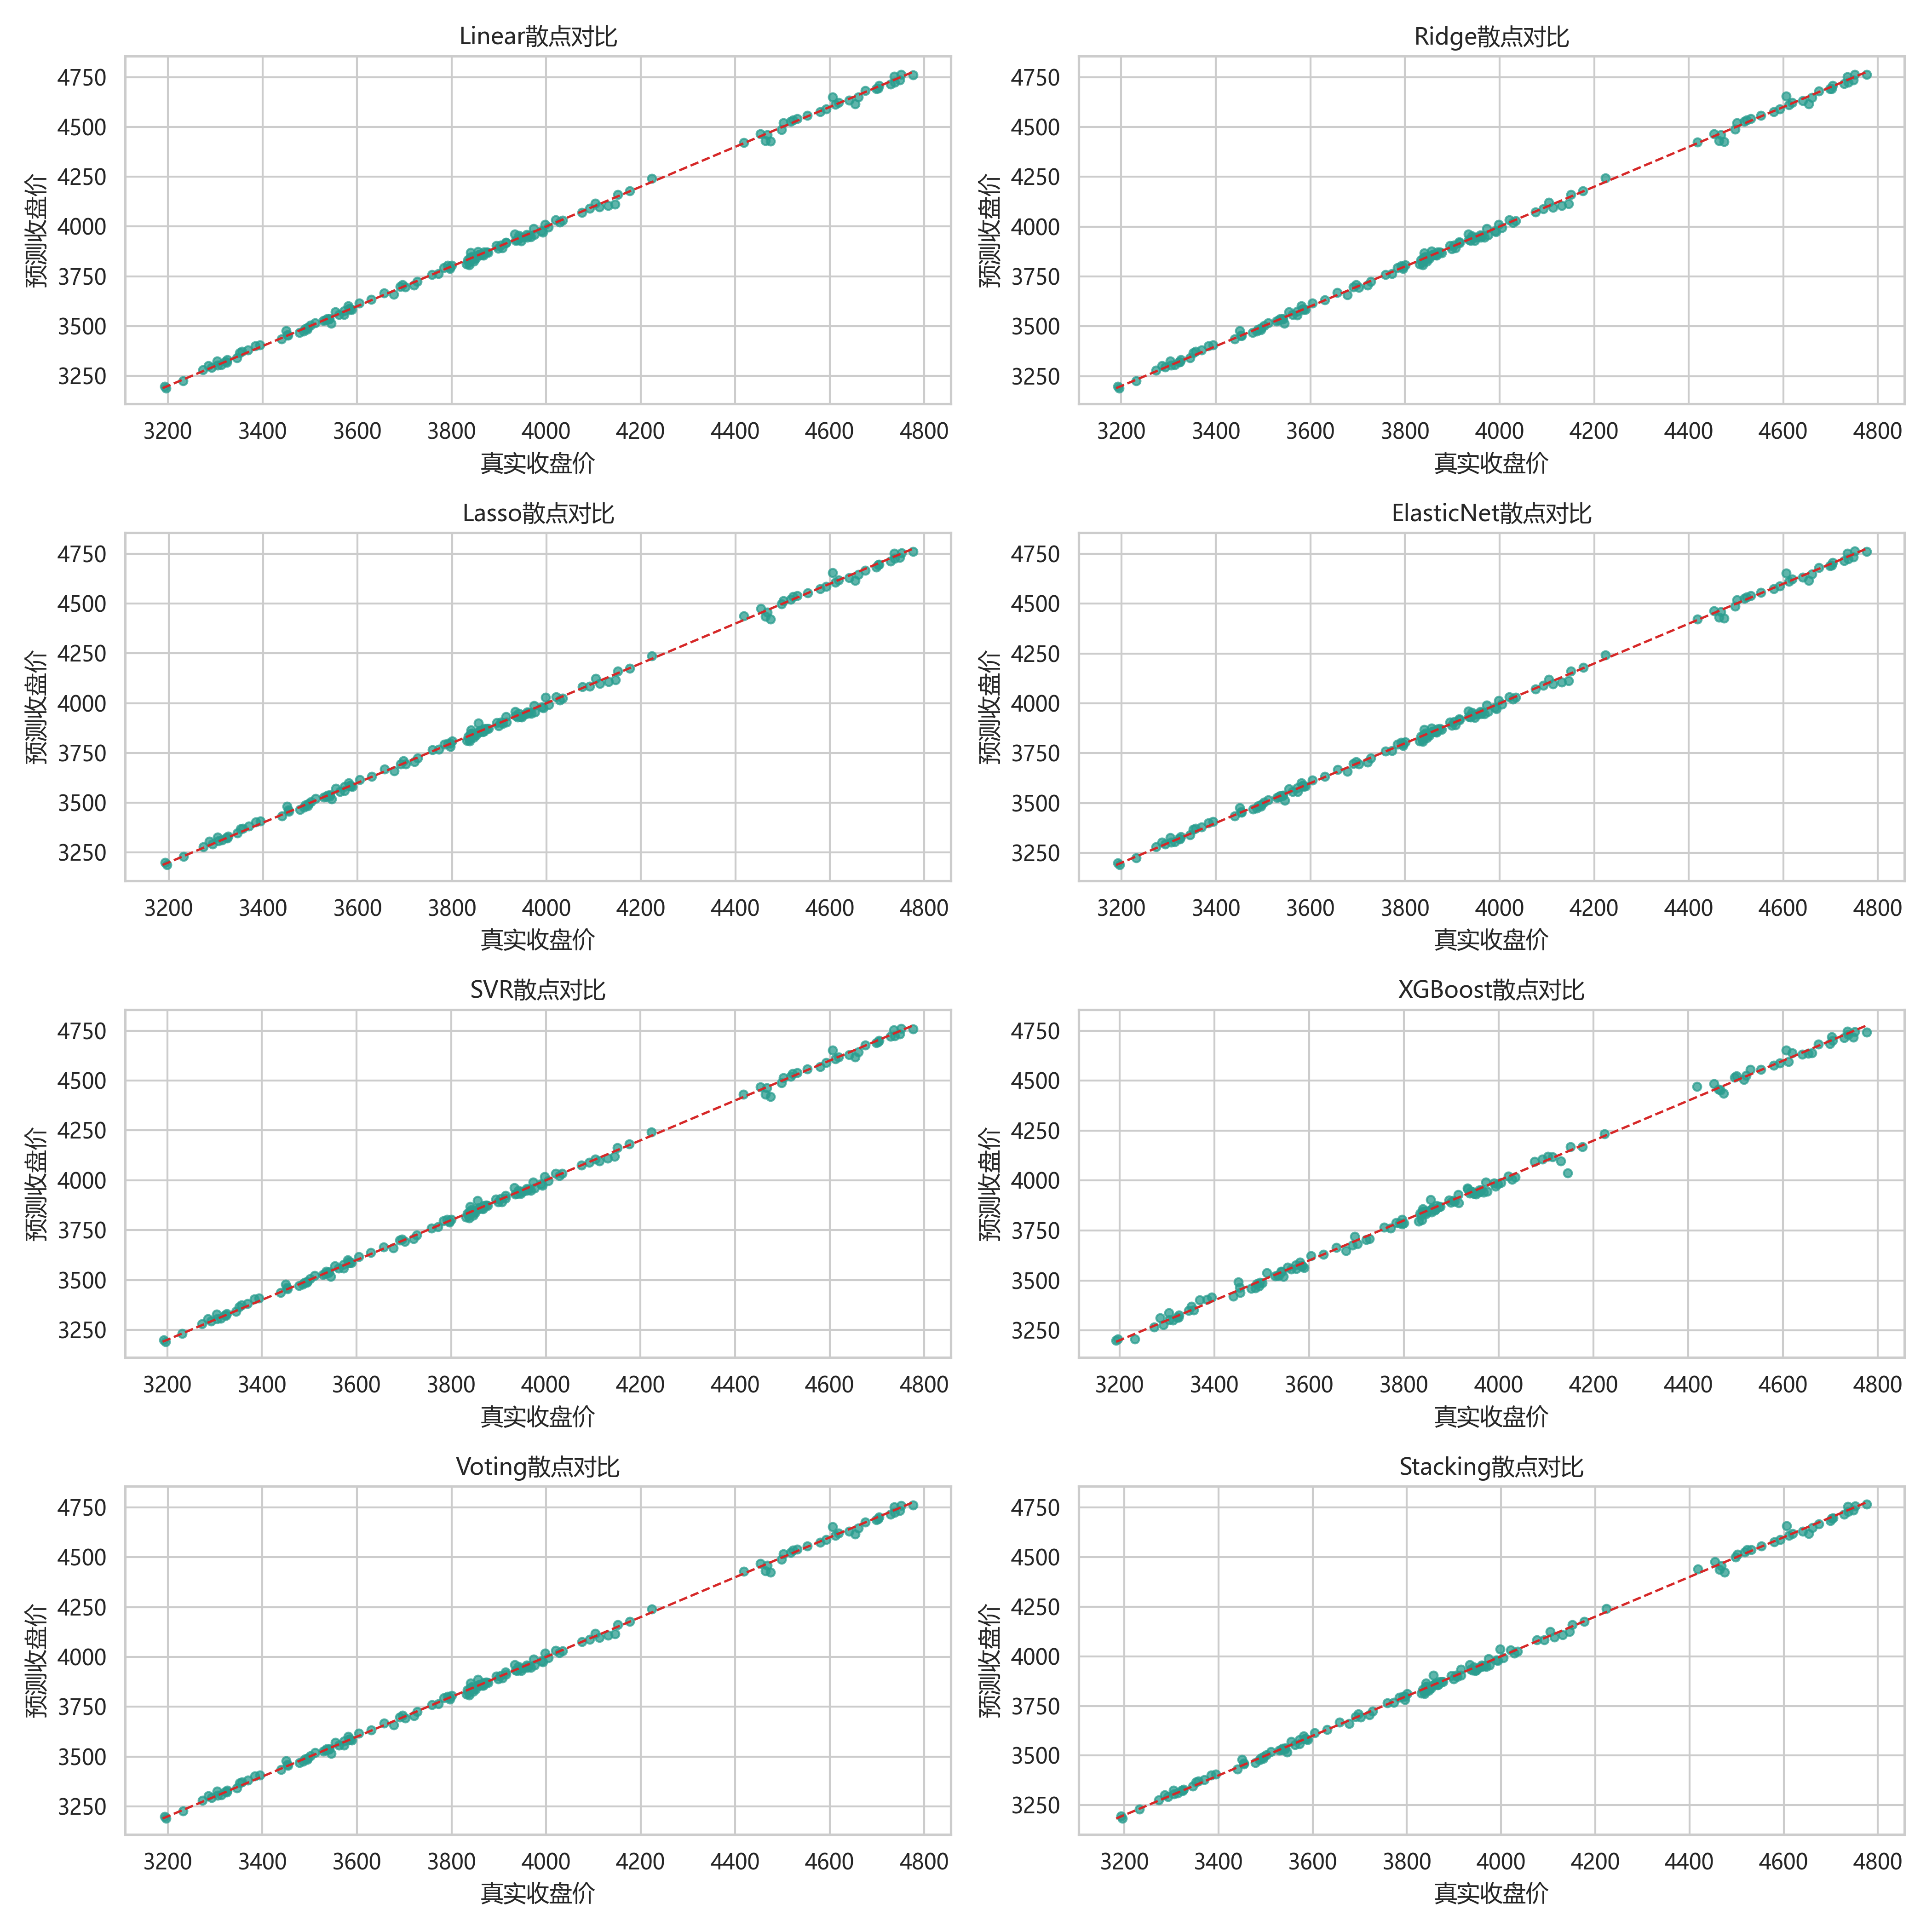
\includegraphics[width=0.94\textwidth]{09_model_prediction_scatter.png}
\caption{各预测模型测试集散点对比}
\label{fig:model-predict-scatter}
\end{figure}

\subsection*{4. 模型预测与评估}
模型训练完成后，使用测试集进行预测，并采用决定系数 $R^2$、均方根误差 RMSE 和平均绝对误差 MAE 对各模型效果进行评价。其中，$R^2$ 越接近 1 表示模型解释能力越强；RMSE 和 MAE 越小，说明预测误差越低。各模型性能对比如表~\ref{tab:metrics} 所示。

\begin{table}[H]
\centering
\caption{各模型性能对比}
\label{tab:metrics}
\begin{tabular}{lcccc}
\toprule
模型 & 训练集$R^2$ & 测试集$R^2$ & 训练集RMSE & 测试集RMSE \\
\midrule
Linear & 0.9989 & 0.9990 & 14.0859 & 13.6981 \\
Ridge & 0.9989 & 0.9990 & 14.1363 & 13.6682 \\
ElasticNet & 0.9989 & 0.9990 & 14.1194 & 13.6753 \\
Voting & 0.9988 & 0.9990 & 14.4013 & 13.7426 \\
SVR & 0.9986 & 0.9989 & 15.9902 & 13.9365 \\
Lasso & 0.9988 & 0.9988 & 14.9313 & 14.5029 \\
Stacking & 0.9985 & 0.9988 & 16.1349 & 14.6430 \\
XGBoost & 0.9998 & 0.9978 & 5.8918 & 20.1172 \\
\bottomrule
\end{tabular}
\end{table}

\begin{figure}[H]
\centering
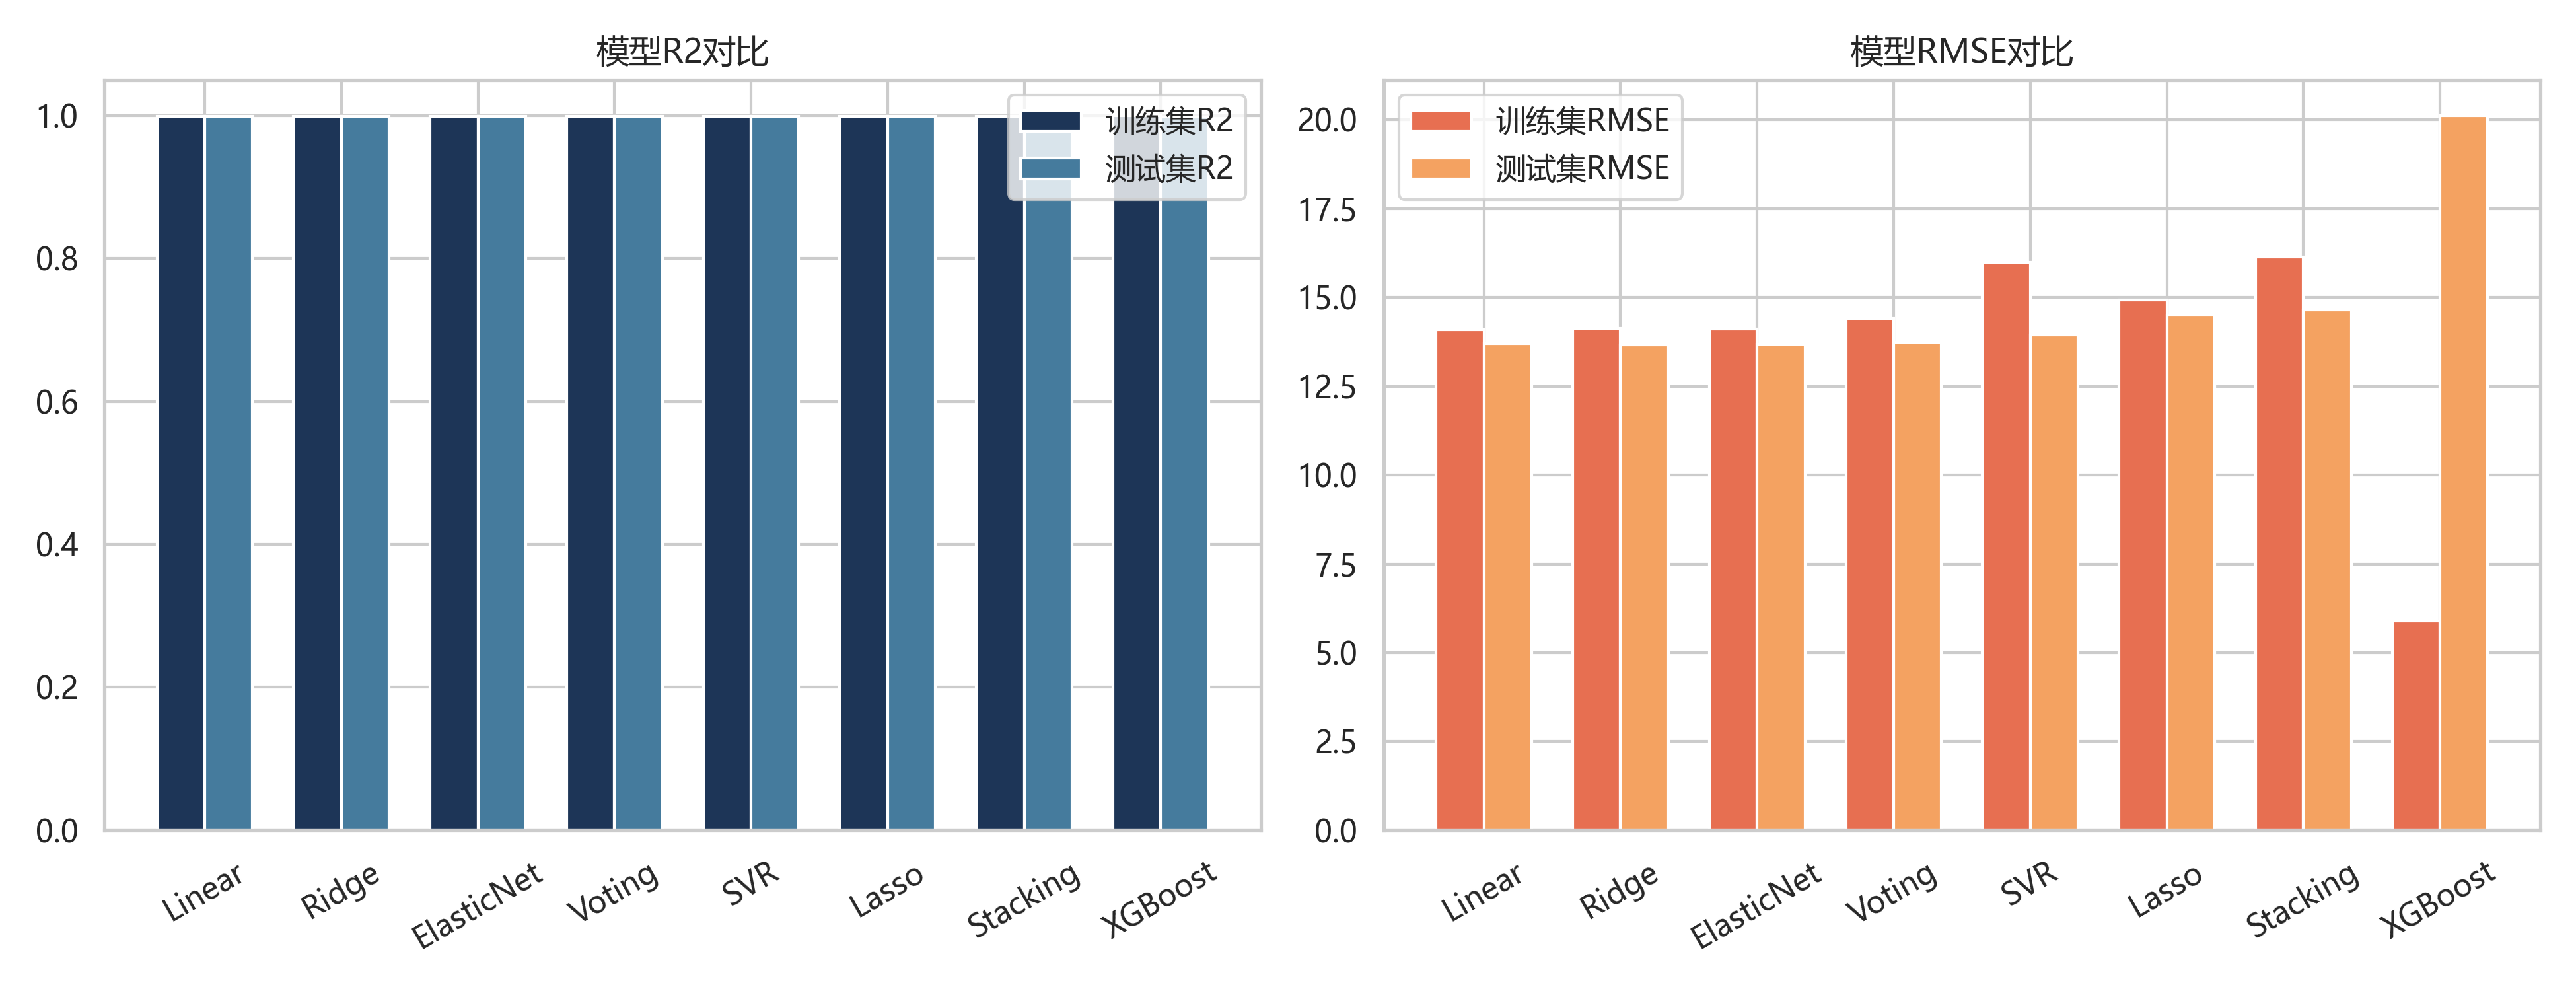
\includegraphics[width=0.86\textwidth]{07_model_comparison.png}
\caption{各模型性能指标综合对比}
\end{figure}

\begin{figure}[H]
\centering
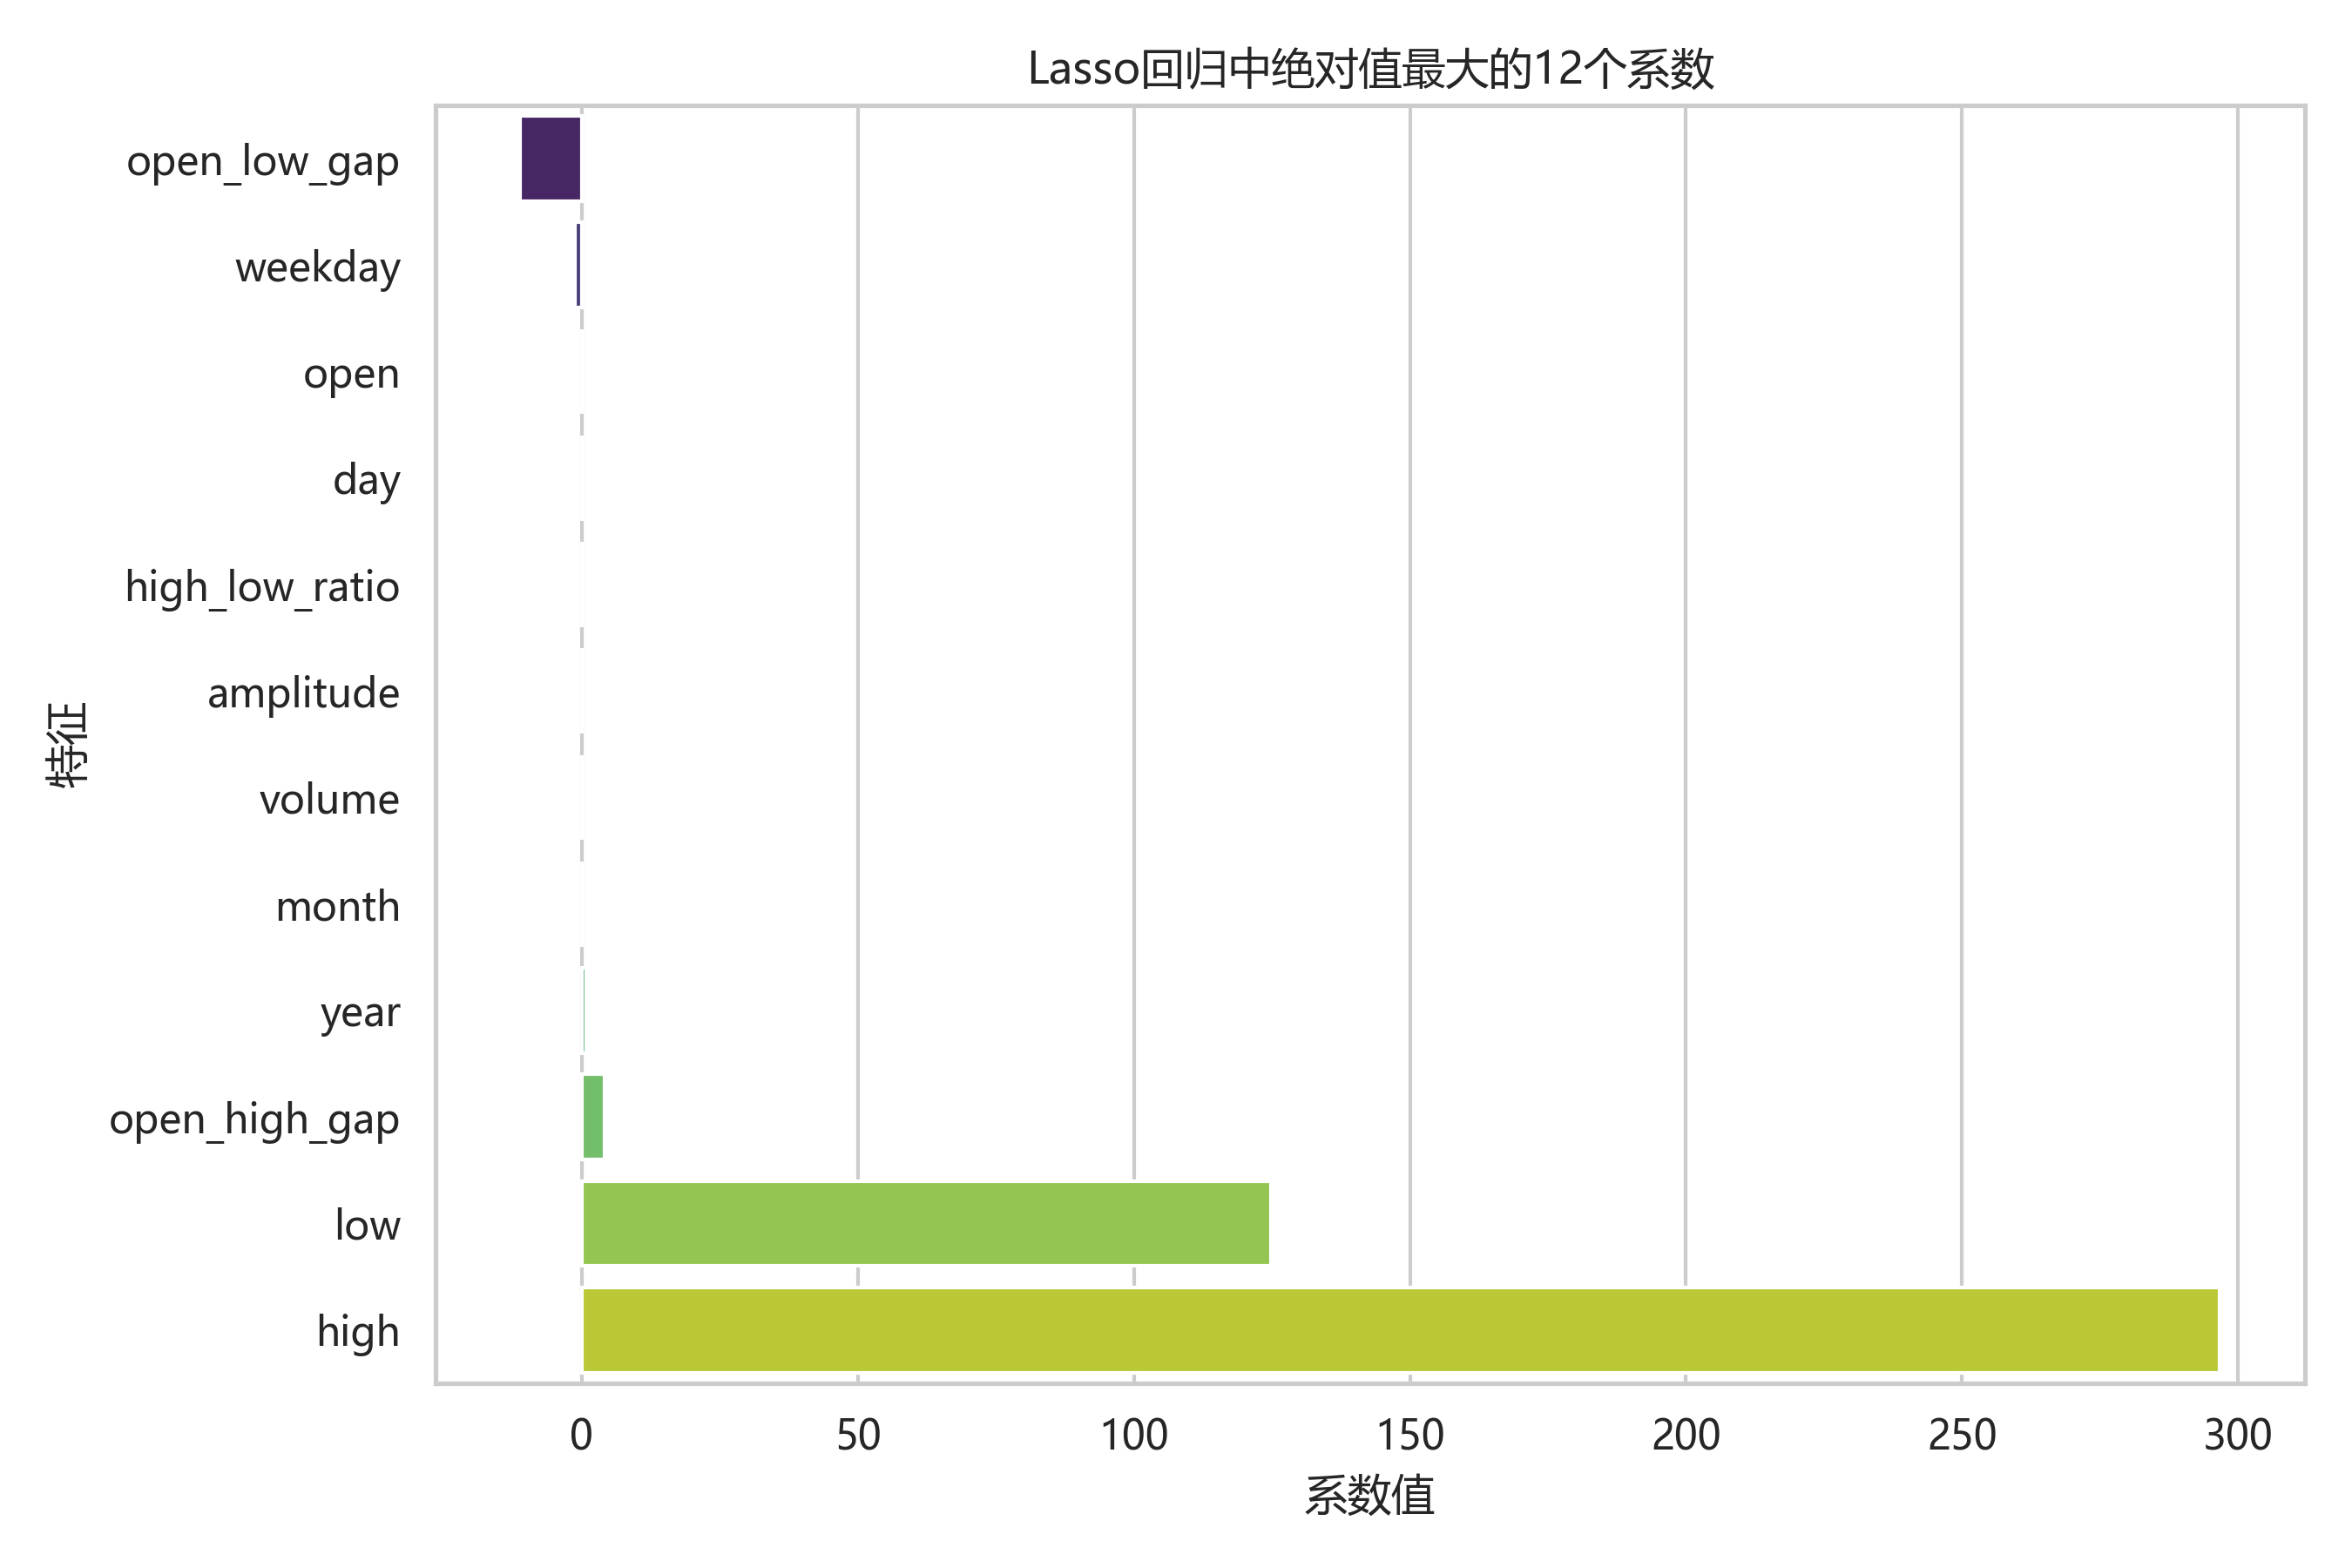
\includegraphics[width=0.72\textwidth]{06_lasso_coefficients.png}
\caption{Lasso 回归重要系数图}
\end{figure}

\subsection*{5. 其他，可选做}
在完成实验基本要求之外，本文还额外保存了模型指标表、全部模型预测值表、Lasso 系数表和最优模型预测结果文件，便于后续整理、复查和再次分析。这些附加结果文件存放在 \texttt{result} 目录下，可直接用于报告撰写和进一步实验扩展。

\section*{五、实验结果与分析}
从表~\ref{tab:metrics} 可以看出，在本次实验中，测试集表现最优的模型为 \textbf{Linear}，其测试集 $R^2$ 达到 0.9990，测试集 RMSE 为 13.6981。这说明经过标准化和较丰富的特征工程后，线性正则化模型在该数据集上具有非常强的拟合能力和泛化能力。

进一步观察不同模型之间的差异，可以发现普通线性回归、Ridge、Lasso、ElasticNet、Voting 和 Stacking 的测试集表现整体都很接近，说明当前数据中的主要关系仍以线性结构为主，正则化和集成方法更多起到增强稳定性、缓解冗余特征影响的作用。其中 Ridge 在测试集上取得最高的 $R^2$，表明 L2 正则化在多重共线性较强的特征环境下具有较好的平衡效果；Lasso 和 ElasticNet 与其差距很小，说明 L1 正则化和混合正则化同样能保持很高的预测精度。

从 Lasso 的系数图可以进一步看出，模型会自动压缩部分系数并保留少数关键特征，体现了 L1 正则化在特征筛选方面的优势。由于本次实验构造了较多价格、成交量和滞后变量，这些特征之间存在较强相关性，因此 Lasso 和 ElasticNet 的引入是有必要的。从最终结果来看，它们既没有明显降低模型表现，又提升了模型解释性。

再看 XGBoost、Voting 和 Stacking 三类模型的表现。XGBoost 在训练集上拟合能力很强，但测试集表现略低于最优线性模型，这说明虽然树模型具有更强的非线性表达能力，但在当前特征结构下并没有占到明显优势。Voting 回归通过平均多个相对稳定的基模型，在测试集上同样取得了很高的 $R^2$，说明简单集成可以有效平滑单个模型的波动。Stacking 回归虽然结构更复杂，但测试表现依旧优秀，说明多层集成策略在本实验数据上是有效的。

结合图~\ref{fig:model-predict-line} 和图~\ref{fig:model-predict-scatter} 可以更直观地发现，不同模型对测试集真实值的跟踪能力存在细微差异。Ridge、Lasso、ElasticNet 和 Voting 的预测曲线与真实曲线贴合度很高，散点也大多分布在对角线附近；XGBoost 的散点离散程度更明显，说明其在部分样本上预测偏差较大。由此可见，在当前任务中，并不是模型越复杂效果就越好，合适的特征工程加上稳定的线性正则化模型往往更有效。

为了进一步说明最优模型的预测质量，本文还对最优模型进行了单独的真实值-预测值散点图和残差分布分析。图~\ref{fig:best-pred} 中样本点大多分布在理想对角线附近，说明预测值与真实值高度一致；图~\ref{fig:best-residual} 显示残差主要集中在 0 附近，整体不存在明显系统偏差，仅在少数样本上存在相对较大的误差。

\begin{figure}[H]
\centering
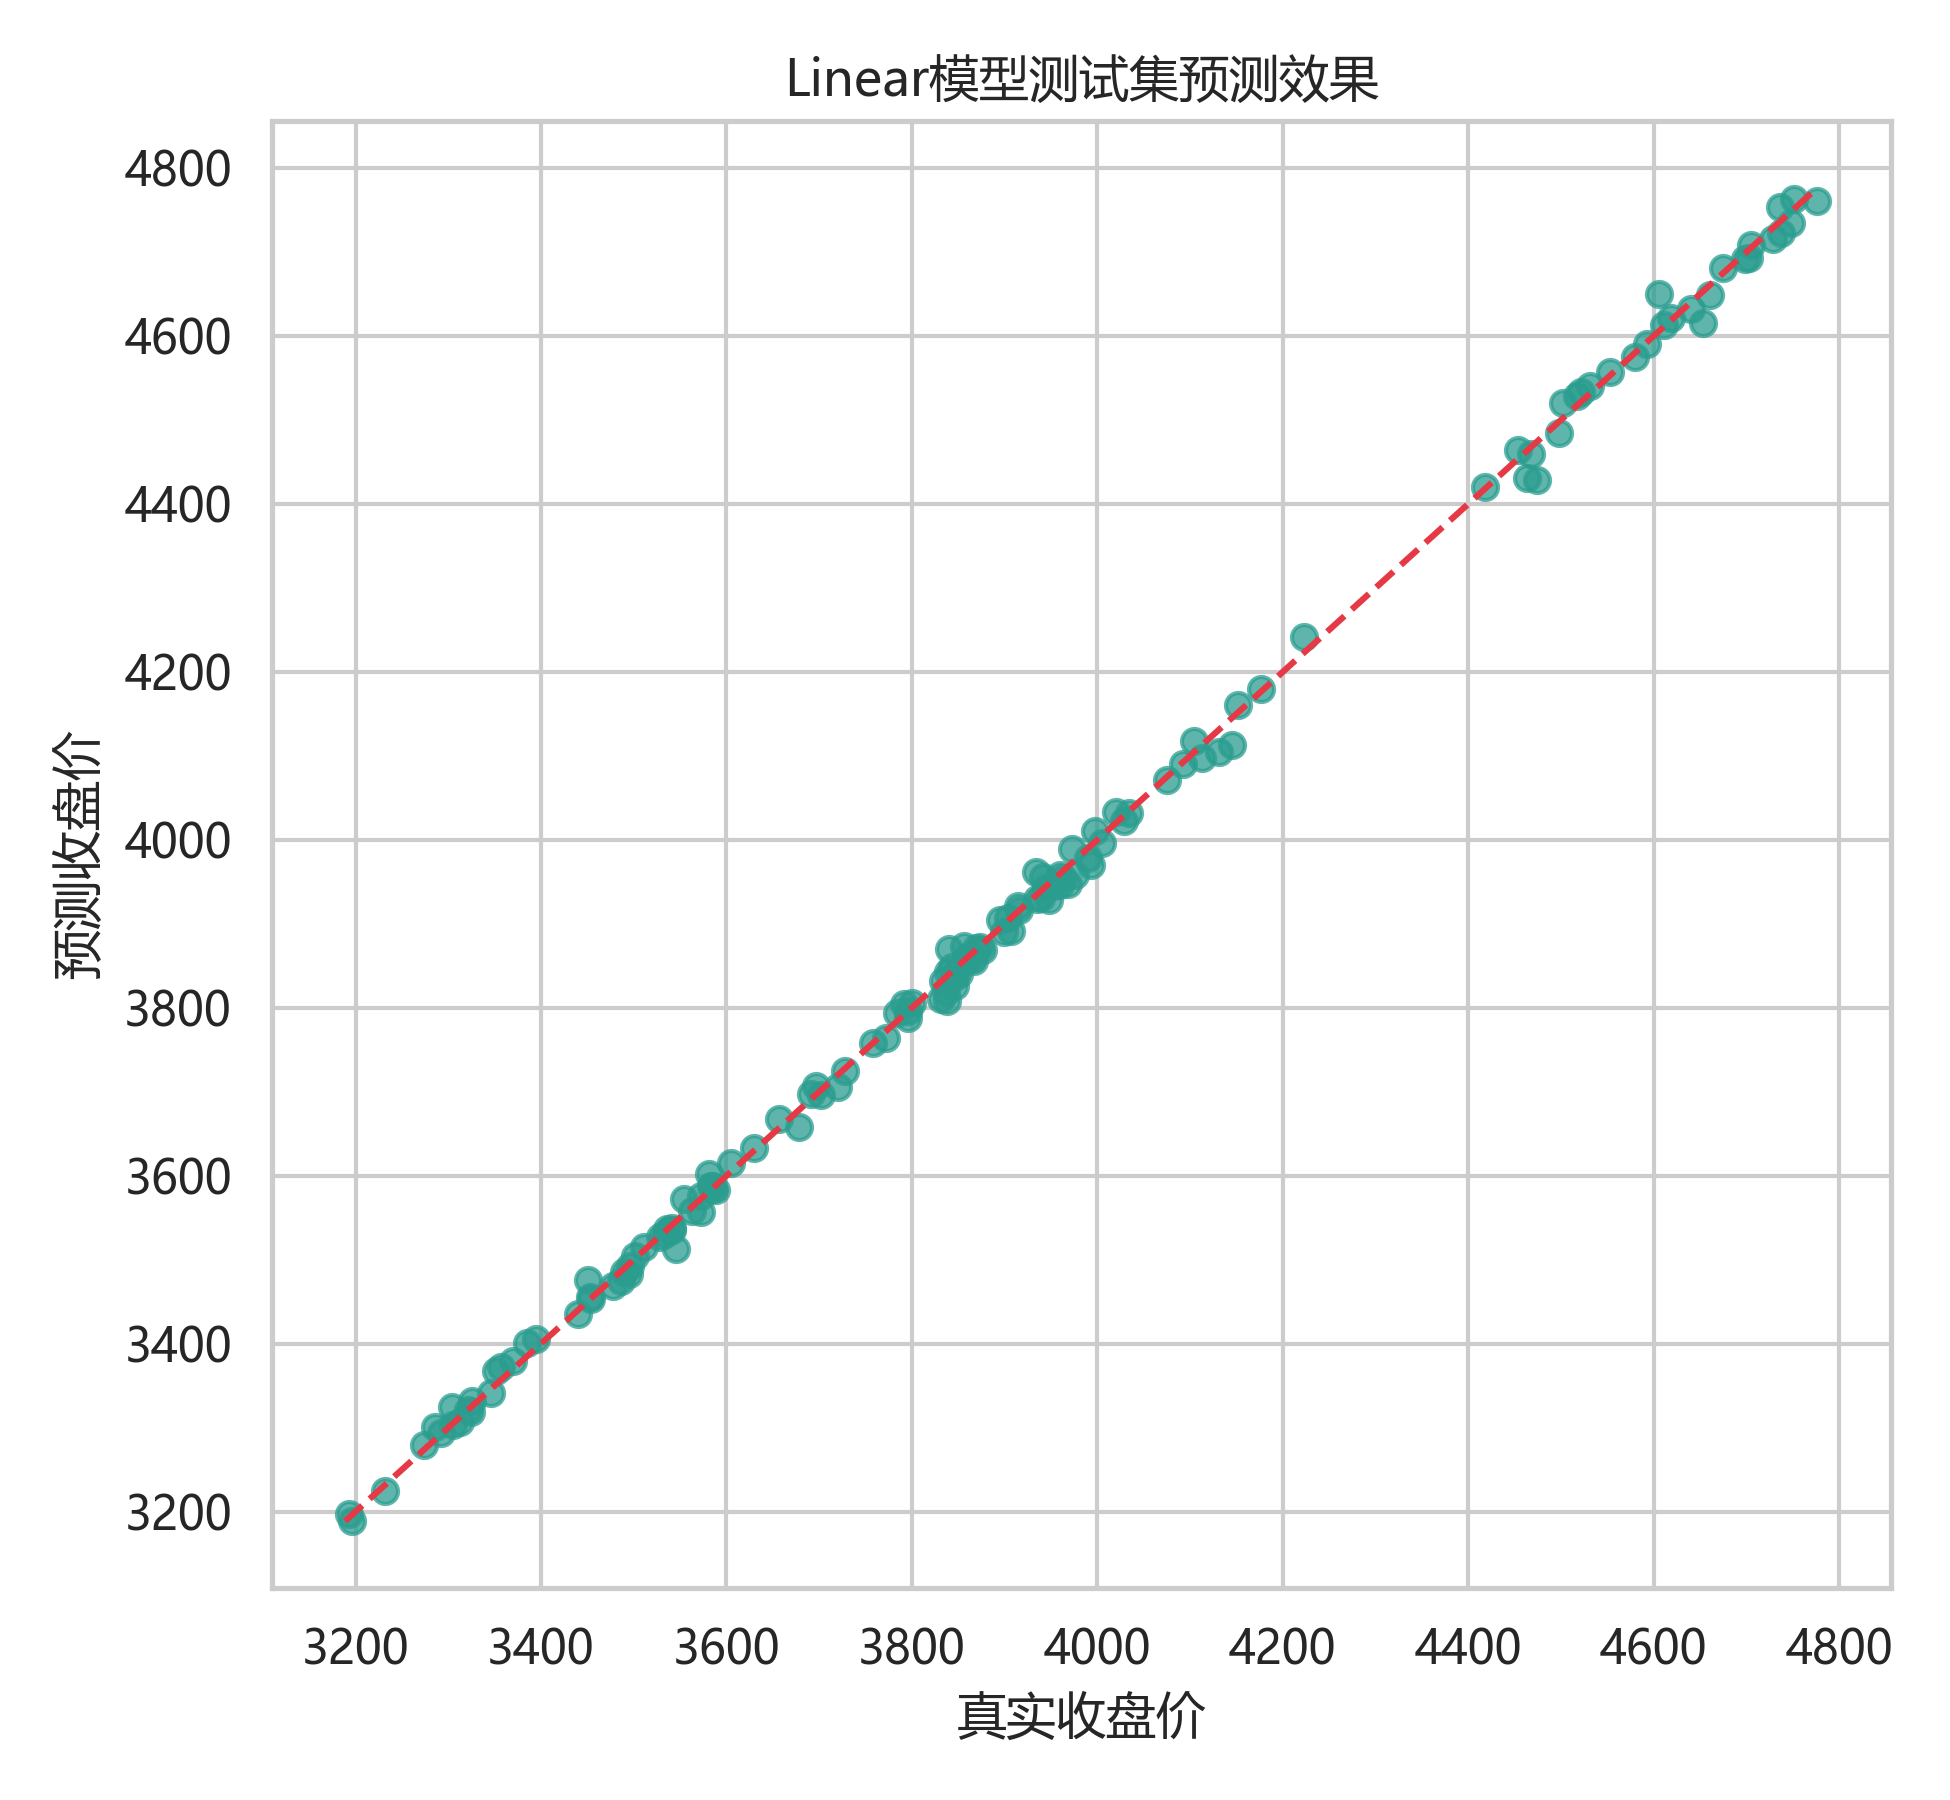
\includegraphics[width=0.68\textwidth]{10_best_model_prediction.png}
\caption{最优模型预测值与真实值对比}
\label{fig:best-pred}
\end{figure}

\begin{figure}[H]
\centering
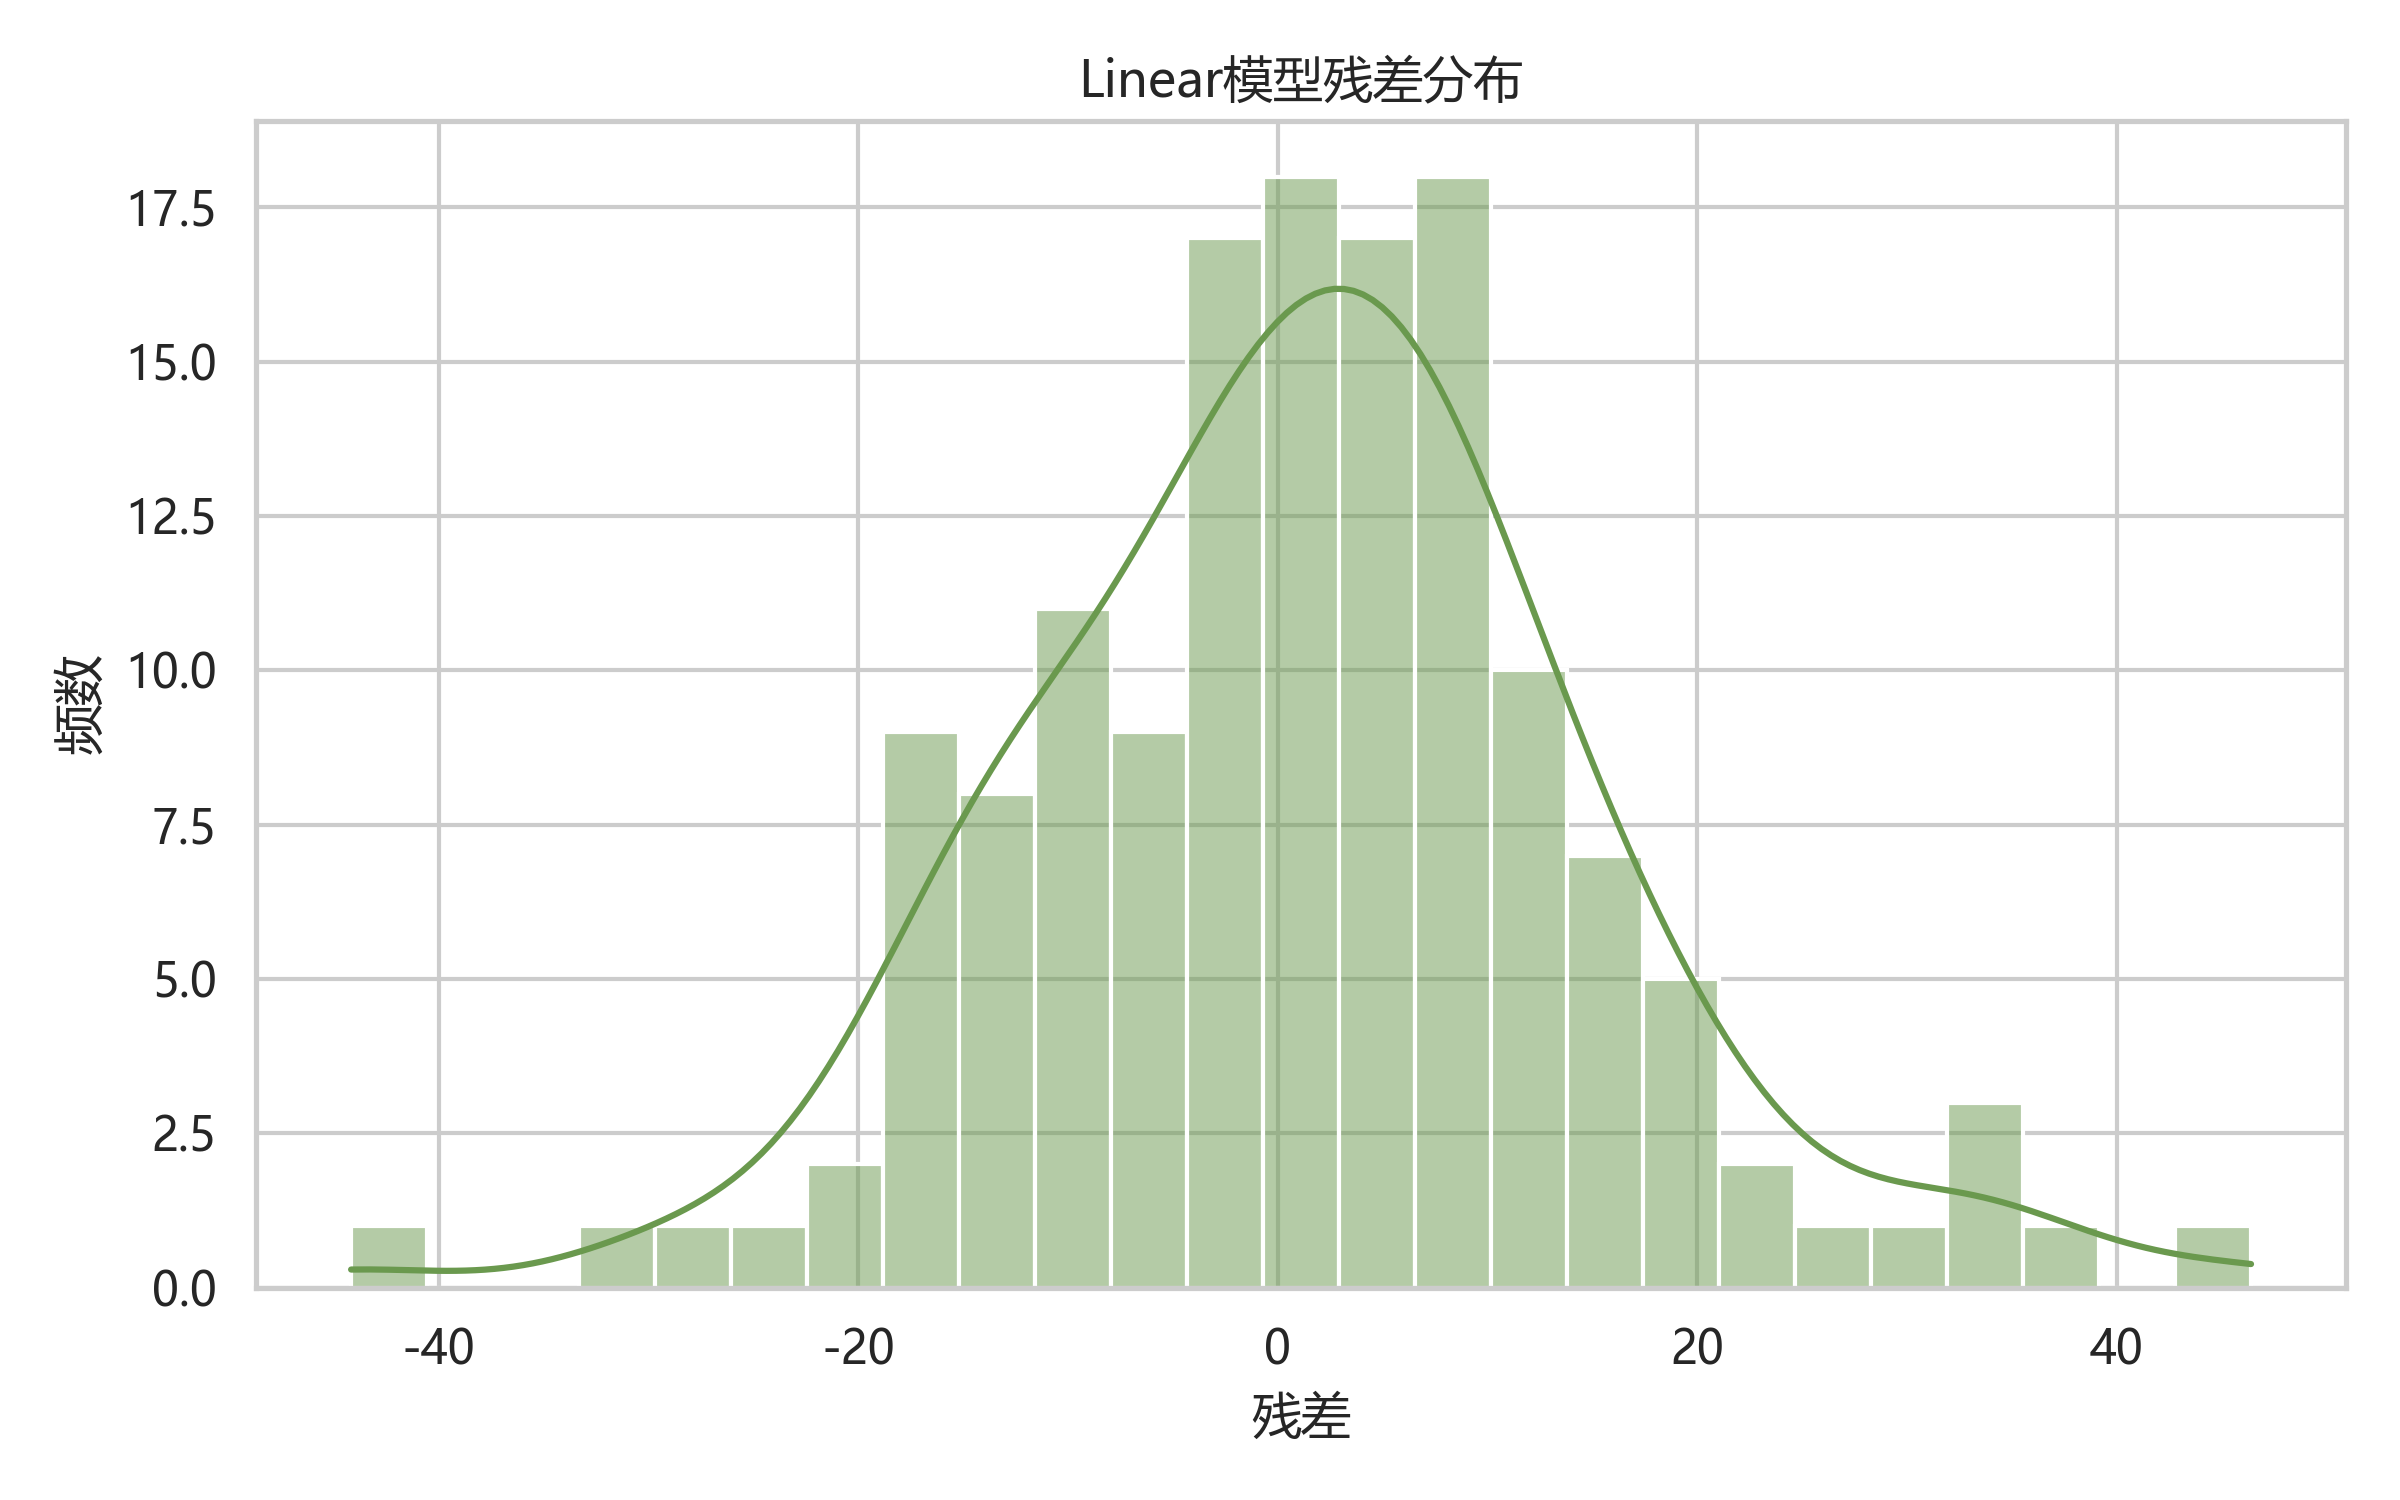
\includegraphics[width=0.75\textwidth]{11_best_model_residuals.png}
\caption{最优模型残差分布}
\label{fig:best-residual}
\end{figure}

总体来看，本次实验说明了三个重要结论。第一，在特征数量较多且存在明显共线性的情况下，Ridge、Lasso 和 ElasticNet 等正则化回归模型是非常有效的选择。第二，标准化处理不仅是实验步骤要求，更是保证正则化公平惩罚各个特征的重要前提。第三，Voting 和 Stacking 等集成学习方法虽然结构更复杂，但是否一定优于正则化线性模型仍然取决于具体数据特征，因此模型选择应以实验结果为依据，而不能仅凭模型复杂度判断优劣。

\section*{六、实验总结}
本次实验围绕“回归模型与模型评估”这一主题，完整实现了数据读取、缺失值处理、异常值处理、特征工程、标准化、模型训练、模型预测、结果可视化和实验报告撰写的完整流程。与实验三相比，本次实验不仅继续强化了数据预处理与特征构造的能力，还进一步扩展到了正则化模型、Boosting 模型和集成学习模型的比较分析。

通过实验，我进一步理解了 Ridge、Lasso 和 ElasticNet 三种正则化方法之间的联系与区别，也体会到特征标准化在正则化模型中的必要性。同时，通过将 XGBoost、Voting 和 Stacking 纳入同一实验框架，我更加清楚地认识到，不同模型各有优势，最终应通过统一的数据集和统一的评价指标进行客观比较。

从实验结果来看，在沪深300近三年的日线数据上，经过适当的特征工程和标准化后，线性正则化模型表现非常稳定，其中 Ridge 模型综合效果最好。这说明面对结构较稳定、线性关系较强的数据场景，简单、可解释且稳健的模型往往比更复杂的非线性模型更实用。后续如果继续拓展本实验，还可以尝试时间顺序划分、滚动窗口验证或更复杂的金融时序特征，以进一步研究模型在更严格预测场景下的表现。

\end{document}
